\documentclass[11pt,a4paper]{article}
\usepackage[utf8]{inputenc}
\usepackage[spanish]{babel}
\usepackage{graphicx}
\usepackage{subcaption}
\usepackage{amsmath,amssymb,amsfonts}
\usepackage{mathtools}
\usepackage{geometry}
\usepackage{xcolor}
\usepackage{hyperref}
\usepackage{booktabs}
\usepackage{enumitem}
\usepackage{fancyhdr}
\usepackage{titlesec}
\usepackage{microtype}
\usepackage{float}
\usepackage{listings}
\usepackage{color}

% Establecer márgenes
\geometry{a4paper, margin=1in, top=1.2in, headheight=15pt}

% Configurar hipervínculos
\hypersetup{
    colorlinks=true,
    linkcolor=blue,
    filecolor=blue,
    citecolor=blue,
    urlcolor=blue,
    pdftitle={Práctica 1},
    pdfauthor={Renato Bedriñana Cárdenas, Hugo Blanco Demelo},
    pdfsubject={Práctica 1 - Sampling and Quantization},
}

% Configuración de encabezado y pie de página
\pagestyle{fancy}
\fancyhf{}
\fancyhead[L]{\footnotesize Práctica 1}
\fancyhead[R]{\footnotesize Sampling and Quantization}
\fancyfoot[C]{\thepage}
\renewcommand{\headrulewidth}{0.4pt}
\renewcommand{\footrulewidth}{0.4pt}

% Configuración para código fuente
\definecolor{codegreen}{rgb}{0,0.6,0}
\definecolor{codegray}{rgb}{0.5,0.5,0.5}
\definecolor{codepurple}{rgb}{0.58,0,0.82}
\definecolor{backcolour}{rgb}{0.95,0.95,0.95}

\lstset{
    backgroundcolor=\color{backcolour},
    commentstyle=\color{codegreen},
    keywordstyle=\color{magenta},
    stringstyle=\color{codepurple},
    basicstyle=\ttfamily\small,
    breakatwhitespace=false,
    breaklines=true,
    captionpos=b,
    keepspaces=true,
    numbersep=5pt,
    showspaces=false,
    showstringspaces=false,
    showtabs=false,
    tabsize=2
}

% Formato de títulos
\titleformat{\section}
  {\normalfont\large\bfseries\color{blue!70!black}}
  {\thesection}{1em}{}
\titleformat{\subsection}
  {\normalfont\normalsize\bfseries\color{blue!60!black}}
  {\thesubsection}{1em}{}

% Espacio después de secciones
\titlespacing*{\section}{0pt}{3.5ex plus 1ex minus .2ex}{2.3ex plus .2ex}
\titlespacing*{\subsection}{0pt}{3.25ex plus 1ex minus .2ex}{1.5ex plus .2ex}

% Definición de comandos para matemáticas
\newcommand{\dB}{\text{dB}}
\newcommand{\dBFS}{\text{dBFS}}

% Información del documento
\title{\vspace{-1.5cm}\Large\textbf{Práctica 1: Sampling and Quantization}}
\author{\normalsize Renato Bedriñana Cárdenas \and \normalsize Hugo Blanco Demelo}
\date{\normalsize\today}
\usepackage[T1]{fontenc}
\usepackage{lmodern}

\begin{document}

\maketitle
\section{Task 1}
\textbf{Question: Give your interpretation of the resulting graphs. Do the quantization levels correspond with the values you had expected?}

\vspace{0.5cm}
We represent the original continuous signal x (blue) and the 2 quantized version using 2 (red) and 4 (yellow) bits. As expected, the 2 bit quantization produces fewer discrete levels than the 4 bits quantization. Increase the number of bits decreases $\Delta$, resulting in smaller steps and a quantized signal that follows the input more closely.

\vspace{1cm}
\textbf{Question: For both cases, represent the quantization error as a function of input amplitude in the range $[-7, +7]$ and comment on your results. Is this error always within the $[-\Delta /2, +\Delta /2]$ interval?}

\vspace{0.5cm}
The magnitude of the error decreases as the number of bits increases, since a smaller quantization step
$\Delta$ reduces the maximum deviation between the input and its quantized version.
The $[-\Delta /2, +\Delta /2]$ in each case is as follows:
\begin{itemize}
    \item For N = 2 the $\Delta$ value we get is $\Delta = 3.5$, so the interval should be $[-1.75, 1.75]$.
    \item For N = 4 the $\Delta$ value we get is $\Delta = 0.875$, so the interval should be $[-0.4375, 0.4375]$.
\end{itemize}
In both cases, the error remains bounded within the theoretical interval $[-\Delta /2, +\Delta /2]$.

\begin{figure}[H]  % H is fot NOT letting latex insert the image in another place
    \centering
    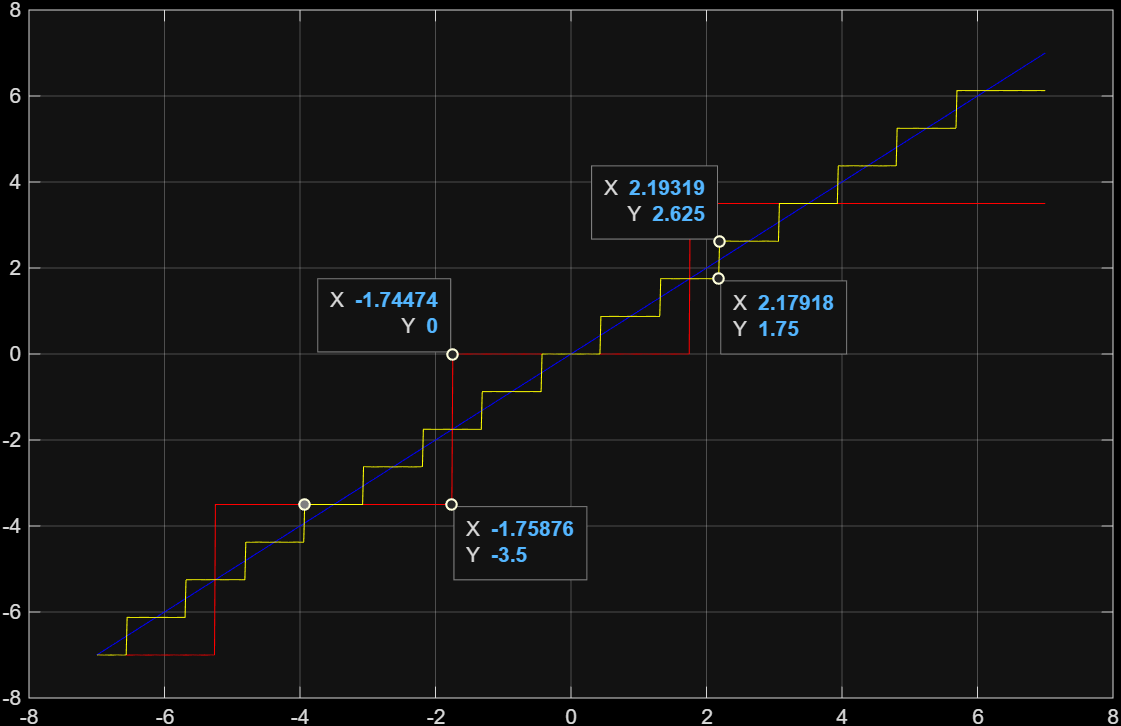
\includegraphics[width=1\textwidth]{img/task1_2.png}
    % \caption{Description of your image}
    \label{fig:task1_2}
\end{figure}

\begin{figure}[H]
    \centering
    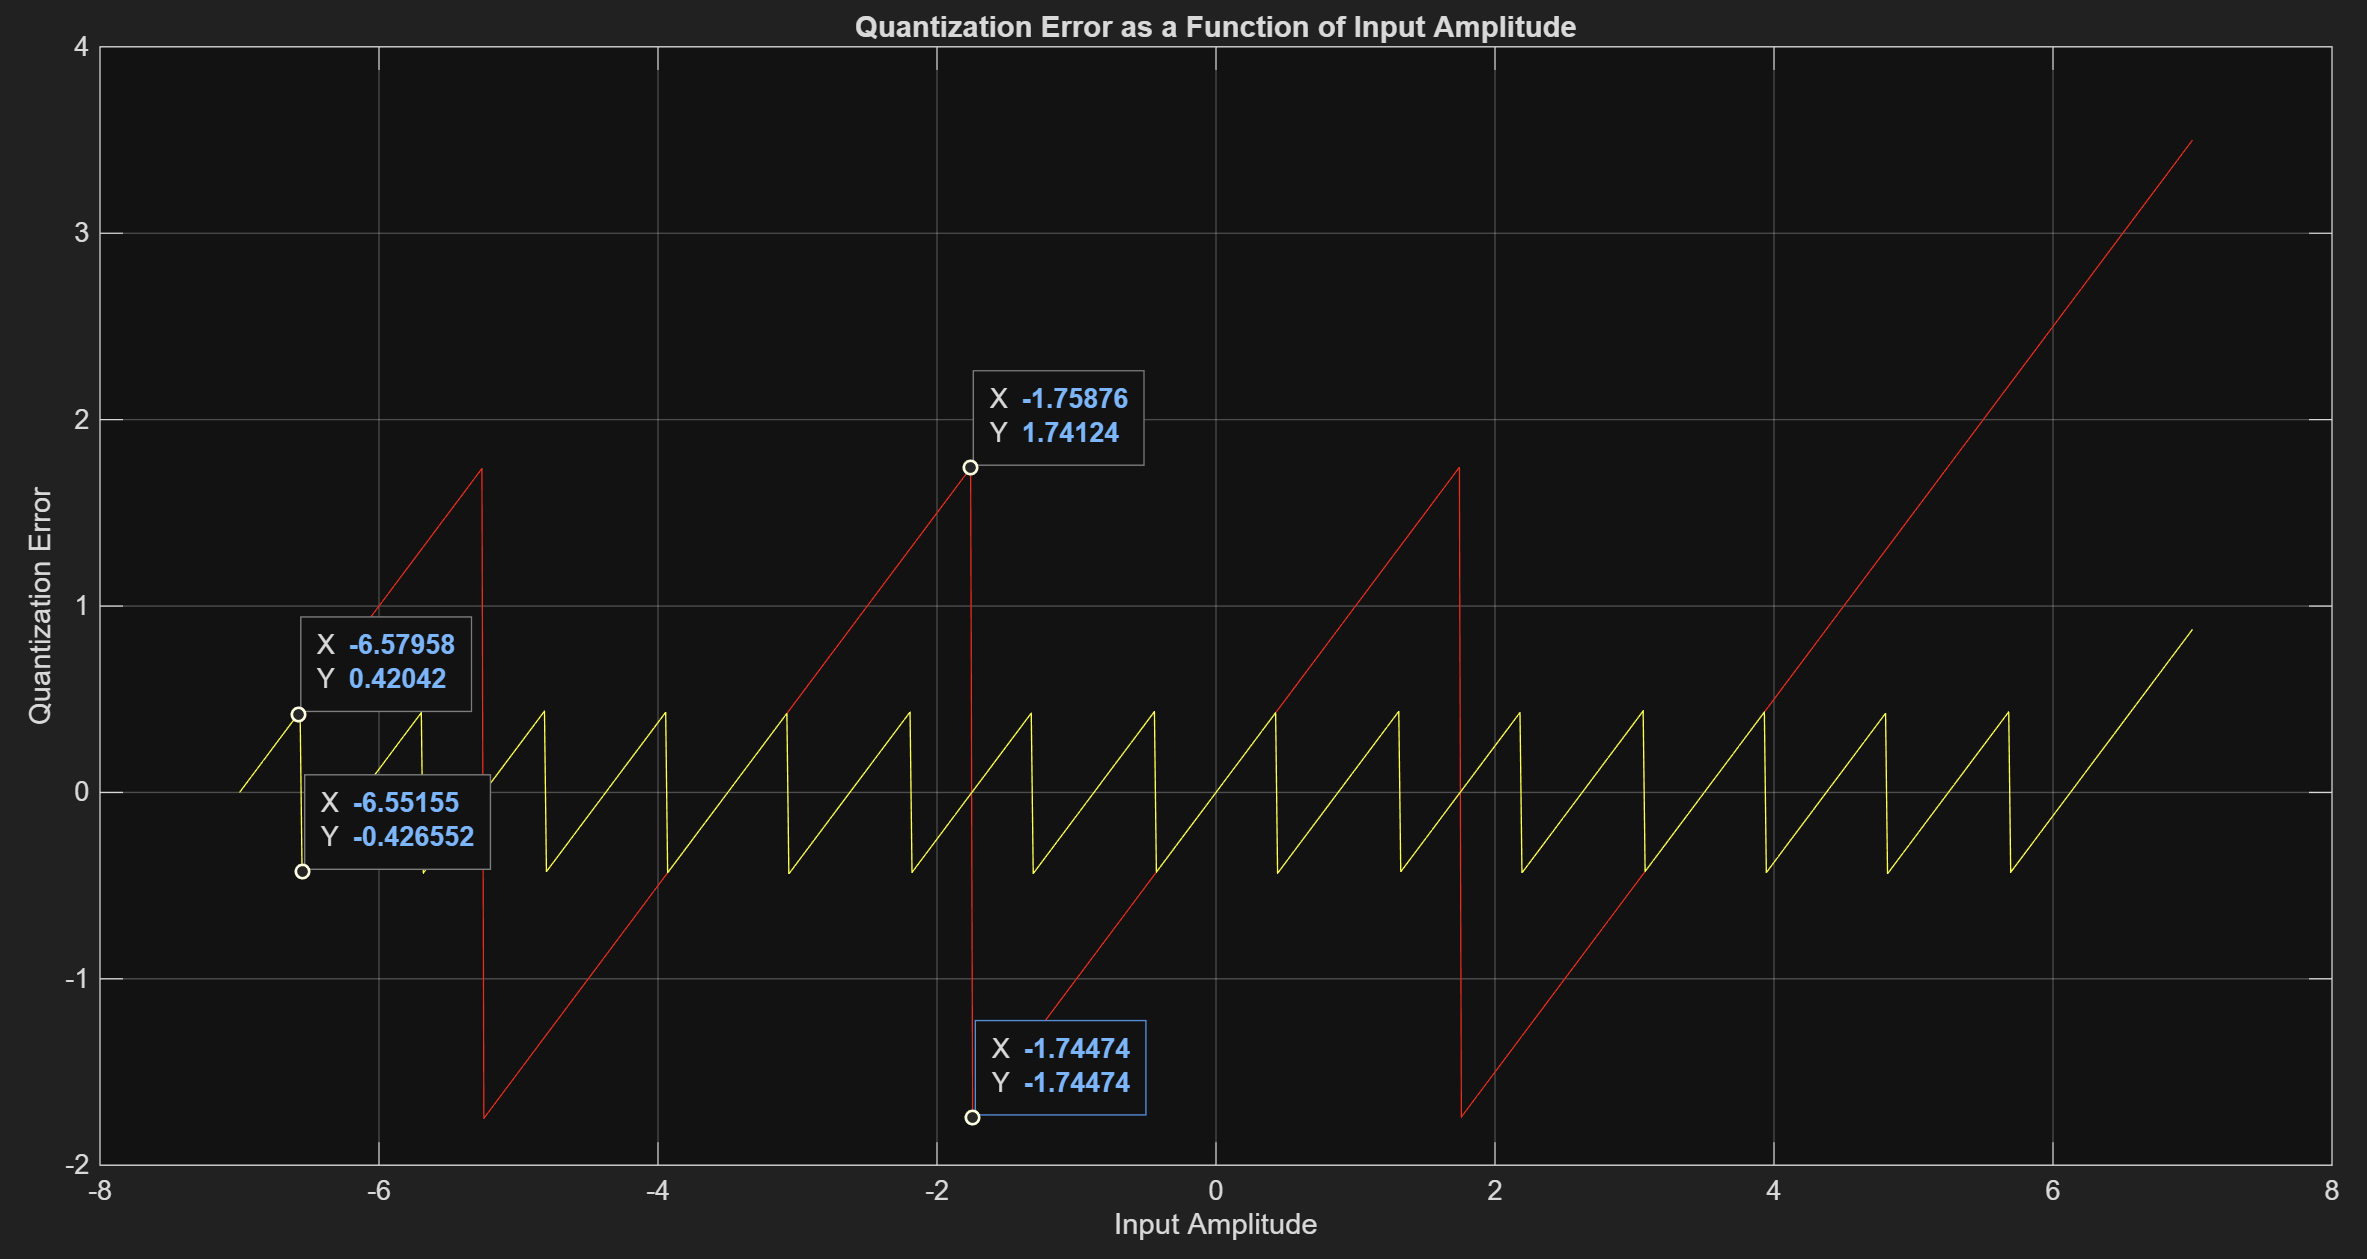
\includegraphics[width=1\textwidth]{img/task1_2_2.png}
    % \caption{Description of your image}
    \label{fig:task1_2_2}
\end{figure}

\section{Task 2}
\textbf{Question: Assume a full-scale sinusoidal input and plot the histogram of the quantization error. Do you observe what you expected, or not?}

\vspace{0.5cm}
Due we have an amplitude equal to FS we can expect clipping. We have $\Delta= \frac{2*FS}{2^N} = 0.0098$, the $[-\frac{\Delta}{2}, +\frac{\Delta}{2}]$ interval should be uniformly distributed (while the input does not get clipped) between $[-0.0049, +0.0049]$.
In the histogram we can see that in that interval the error is uniformly distributed, but there is an error tail in the positive extreme.
It means that there is \textbf{clipping} in the positive.

\begin{figure}[H]
    \centering
    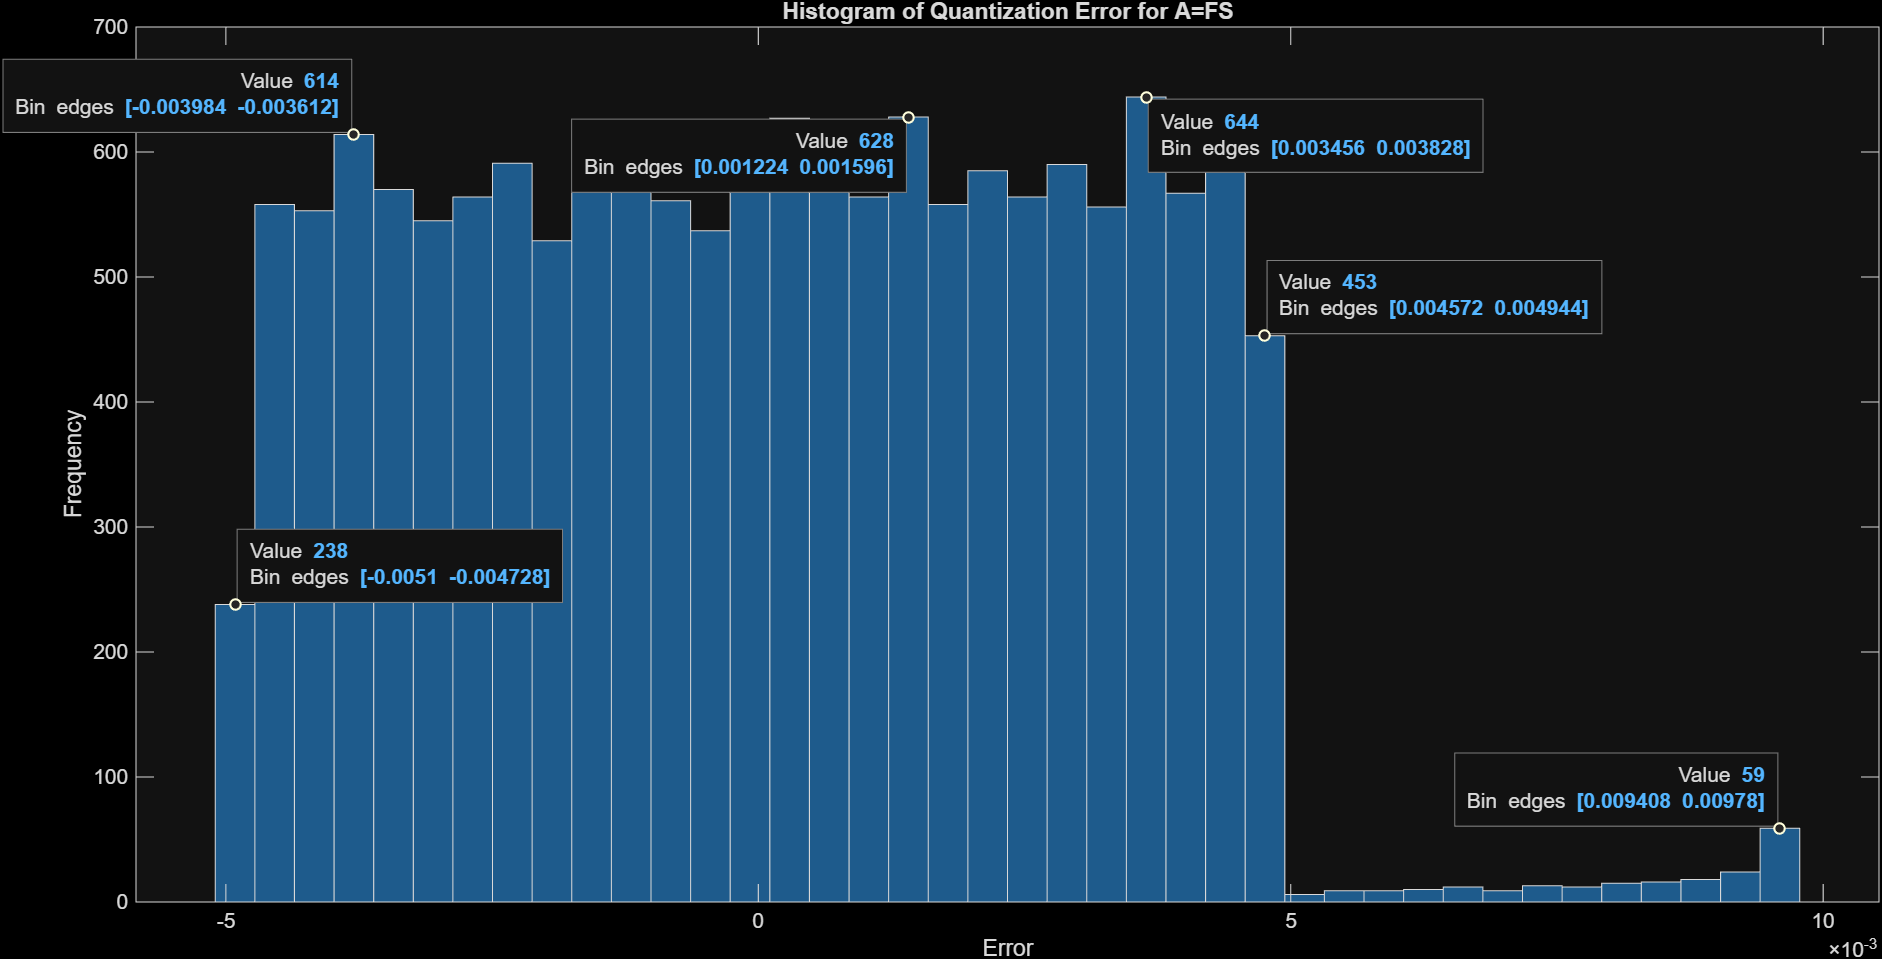
\includegraphics[width=1\textwidth]{img/task2_1.png}
    % \caption{Description of your image}
    \label{fig:task2_1}
\end{figure}

\vspace{1cm}
\textbf{Question: Explain the operation of the Matlab command var. Estimate the variance of the quantization error using var,
    and compare it to its theoretical value. Estimate the value (in dB) of the Signal to-Quantization Noise Ratio (SQNR)
    and compare it to its theoretical value.
}

\vspace{0.5cm}
The MATLAB command \texttt{var} computes the variance of a set of values. For a vector $x$, it calculates:
$\text{var}(x) = \frac{1}{n-1}\sum_{i=1}^n (x_i - \bar{x})^2$, where $\bar{x}$ is the mean of the values in $x$ and $n$ is the total number of samples.
We used \texttt{var(x,1)} to compute the population variance (divide by n).

The empiral value of the variance of the quantization error we got is $8.72123e-06$, and the theoretical value is $\frac{\Delta^2}{12} = 7.94729e-06$.

The estimated value of the SQNR in dB we got is $61.5633$ dB, and the theoretical value is $61.9597$ dB.

\vspace{1cm}
\textbf{Question: Repeat the previous steps for sinusoids with different amplitudes, and with decreasing resolutions
    of 12, 10, 8, 6 and 4 bits, in order to fill Table 1, rounding the SQNR values (in dB) to two
    decimal places. Comment on your results.
}

\vspace{0.5cm}
\begin{table}[H]
    \centering
    \begin{tabular}{|c||c|c|c|c|c|c|c|c|}
        \hline
                    & \multicolumn{2}{c|}{$A=0.5\cdot\text{\tt FS}$} & \multicolumn{2}{c|}{$A=0.75\cdot\text{\tt FS}$} & \multicolumn{2}{c|}{$A=\text{\tt FS}$} & \multicolumn{2}{c|}{$A=1.03\cdot\text{\tt FS}$}                                          \\
        \cline{2-9} & \multicolumn{2}{ |c| }{SQNR (dB)}              & \multicolumn{2}{ |c| }{SQNR (dB)}               & \multicolumn{2}{ |c| }{SQNR (dB)}      & \multicolumn{2}{ |c| }{SQNR (dB)}                                                        \\
        \hline
        $N$         & theory                                         & measured                                        & theory                                 & measured                                        & theory  & measured & theory & measured \\
        \hline\hline
        12          & 67.98                                          & 68.03                                           & 71.5                                   & 71.54                                           & 74.00   & 73.7     & 74.26  & 38.47    \\
        \hline
        10          & 55.94                                          & 56.01                                           & 59.46                                  & 59.53                                           & 61.96   & 61.56    & 62.22  & 38.19    \\
        \hline
        8           & 43.90                                          & 44.04                                           & 47.42                                  & 47.53                                           & 49.92   & 49.15    & 50.18  & 36.97    \\
        \hline
        6           & 31.86                                          & 32.13                                           & 35.38                                  & 35.6                                            & 37.88   & 36.52    & 38.14  & 32.27    \\
        \hline
        4           & 19.82                                          & 20.37                                           & 23.34                                  & 23.78                                           & 25.8397 & 23.63    & 26.1   & 22.53    \\
        \hline
    \end{tabular}
    \caption{Pertaining to Task 2.}
    \label{tab:task2}
\end{table}

For amplitudes below FS (0.5*FS and 0.75*FS) the empirical SQNR values closely match the theoretical predictions.
For an amplitude equal to FS, the empirical values still align well with theory, indicating minimal clipping effects.
However, as the amplitude exceeds FS (1.03*FS), discrepancies arise due to clipping effects, SQNR collapses and even adding more bits does not solve the problem.

As the number of bits decreases the variance of the error grows roughly as expected and SQNR drops approximately 6 dB/bit.
For moderate amplitudes the theory remains a good approximation down to mid-low N (but deviations increases as N gets smaller).

\section{Task 3}
\textbf{Question: Suppose that you have an N-bit A/D converter with tunable FS, and you know that your input samples follow
    a symmetric triangular pdf in some interval $[-x_0,x_0]$. Intuitively, how would you set the FS value of your converter?
    What would the resulting rms value $\sigma_x$ in dBFS be?
}

\vspace{0.5cm}
If you set $FS < x_0$ any imput $|x|$ greater than FS will be clipped. If $FS > x_0$,we would be wasting the converter's since the signal would never
reach the limits. Therefore, the value of FS should be $x_0$.

To reach the variance of a symmetric triangular distribution we need to make some calculations:
\[
    Var(x) = E[x^2] - (E[x])^2 = E[x^2] + 0 = \int_{-x_0}^{x_0} x^2 f(x) dx = x_0^2/6
\]

$\sigma_x = \sqrt{var(x)} = \frac{x_0}{\sqrt{6}}$ and in dBFS (with $x_0$ = FS) would be $20\log_{10}(1/\sqrt{6}) = -7,78$ dBFS.

\vspace{1cm}
\textbf{Question: Explain how to generate in Matlab samples of a random variable following a symmetric triangular pdf with
    zero mean and rms value $\sigma_x$. Check the histogram and use the commands mean and var to validate your approach
}

\vspace{0.5cm}
We have two options to do it:
\begin{itemize}
    % uso task3_2.m
    \item Option 1: The easiest way to generate a random variable with triangular pdf is using the function \textit{makedist} from Matlab.
          The function spects the parameters A, B and C that define the triangular distribution.
          So we set the function parameters to get a symmetric triangular distribution centered at 0: \texttt{makedist('Triangular','A',-x0,'B',x0,'C',0)}

          The result of the mean and var commands are as follows:
          \begin{itemize}
              \item Empirical mean: -4.58885e-05, wich is near to 0, very close to our target mean.
              \item Empirical rms value [dBFS]: -7.78072, wich is very close to our target variance.
          \end{itemize}

          \begin{figure}[H]
              \centering
              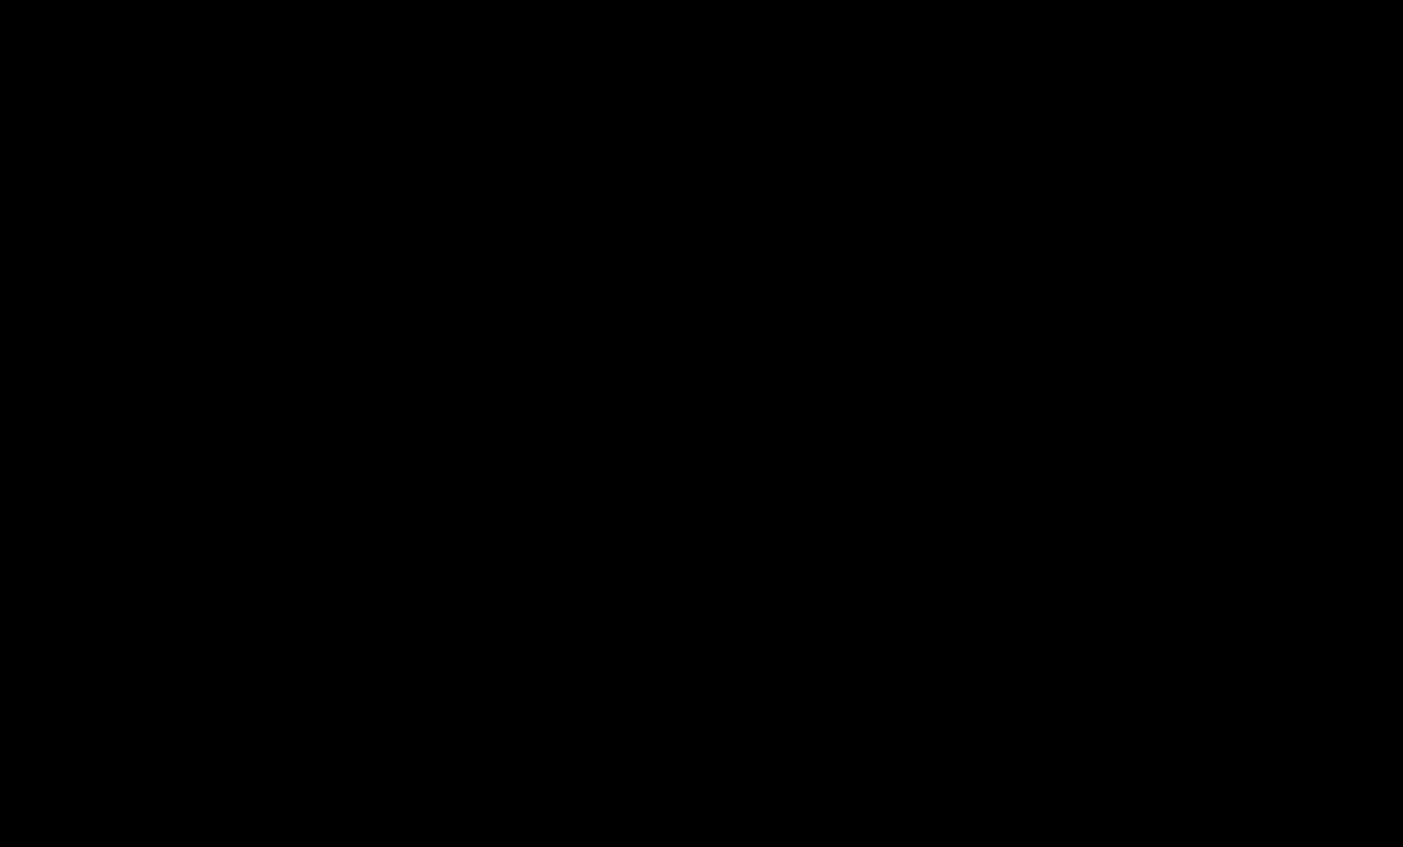
\includegraphics[width=1\textwidth]{img/task3_tri_mkdist.png}
              \label{fig:task3_tri_mkdist}
          \end{figure}

          To do it, we can use the following code:
          \begin{lstlisting}[language=Matlab]
            x0 = 2;
            A = -x0; B = 0; C = +x0; % simetria = media 0

            pd = makedist('Triangular','A',A,'B',B,'C',C);
            N = 100000;
            samples = random(pd, N, 1);

            % comprobaciones rapidas
            emp_mean = mean(samples);
            emp_var = var(samples);
            emp_desv_std = std(samples);

            % valores teoricos
            % theo_mean = 0; % simetria centrado en 0
            theo_var = (A^2 + B^2 + C^2 - A*B - A*C - B*C)/18;
            rms = 20*log10(sqrt(theo_var)/x0);

            fprintf('Theorical mean: 0; emp mean: %.2f\n',emp_mean);
            fprintf('Theorical var: %.2f; emp var: %.2f\n',theo_var,emp_var);
            fprintf('Sigma value: %.2f\n',sqrt(theo_var));
            fprintf('rms value in dBFS: %.2f\n',rms)

            % ver histograma y pdf teorica
            xgrid = linspace(A,C,500)';
            figure
            histogram(samples,100,'Normalization','pdf')
            hold on
            plot(xgrid, pdf(pd,xgrid), 'LineWidth',1.5)
            title('Triangular (media 0) -- muestras vs PDF')
            hold off
        \end{lstlisting}

          % uso task3_tri.m
    \item Option 2: Another way we can generate samples of a random variable following a symmetric triangular pdf as the sum of two independent random variables $X_1$ and $X_2$ from a uniform distribution.
          When two independent random variables with uniform distributions are added, the resulting probability density function (PDF) becomes triangular. This can be understood both intuitively and mathematically.

          Intuitively, if each variable is uniform on \([-a,a]\), there are many pairs that sum near zero but only a few that produce sums near the extremes \(\pm 2a\). Hence the PDF peaks at zero and decreases linearly towards the edges.

          Mathematically, let \(Z = X_1 + X_2\) with \(X_1,X_2\) independent and uniform on \([-a,a]\). The PDF of \(Z\) is the convolution of the two uniform PDFs:
          \[
              f_Z(z) = (f_{X_1} * f_{X_2})(z) = \int_{-\infty}^{\infty} f_{X_1}(t)\, f_{X_2}(-t + z)\, dt.
          \]
          Carrying out the convolution yields the triangular PDF supported on \([-2a,2a]\):
          \[
              f_Z(z) = \frac{2a - |z|}{4a^{2}}, \qquad |z|\le 2a.
          \]
          If we want the triangular distribution to have support \([-x_0,x_0]\), we must choose \(a = x_0/2\). In that case the PDF simplifies to
          \[
              f_Z(z)=\frac{x_0 - |z|}{x_0^2}, \qquad |z|\le x_0,
          \]
          Adding two uniform random variables with 0 mean, results in another random variable with 0 mean.

          \[
              E[Z] = E[X_1 + X_2] = E[X_1] + E[X_2] = 0 + 0 = 0.
          \]

          The variance of the sum of two independent random variables is the sum of their variances.
          So if we want a triangular distribution with variance $\sigma_x$ (in dBFS), we need to set the variance of each uniform variable to $\sigma_x/2$.

          \[
              Var(Z) = Var(X_1 + X_2) = Var(X_1) + Var(X_2) = \sigma_x/2 + \sigma_x/2 = \sigma_x.
          \]

          For a uniform on \([-a,a]\) we have \(\mathrm{Var}(X_i)=a^{2}/3\). Taking \(a=x_0/2\) gives \(\mathrm{Var}(Z)=2\cdot (x_0/2)^2/3 = x_0^2/6 = \sigma_x\), as required.

          The result of the mean and var commands are as follows:
          \begin{itemize}
              \item Empirical mean: 0.00003, wich is close to 0, very close to our target mean.
              \item Empirical variance [dB]: -7.80701, wich is very close to our target variance.
          \end{itemize}

          \begin{figure}[H]
              \centering
              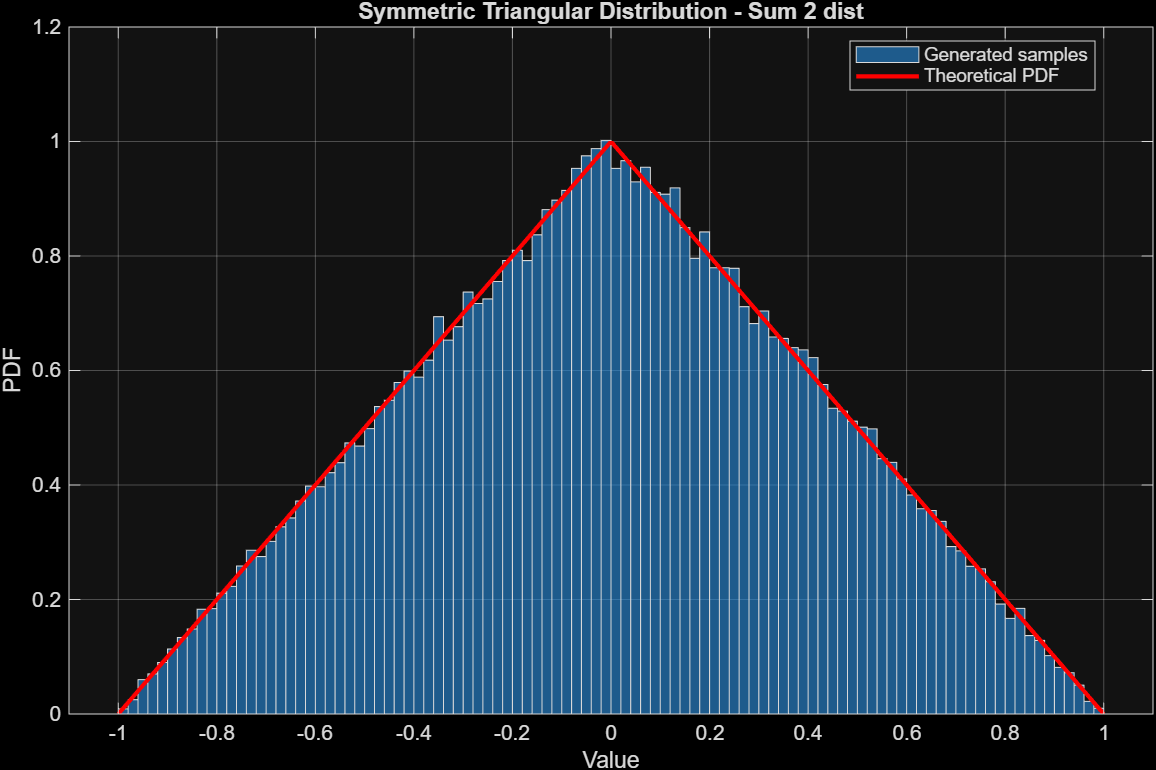
\includegraphics[width=1\textwidth]{img/task3_tri_sum2uniform.png}
              \label{fig:task3_tri_sum2uniform}
          \end{figure}

          we can doit as follows: REVISAR!!
          \begin{lstlisting}[language=Matlab]
            x0=2;
            sigma0 = x0/sqrt(2);
            N = 100000;
            
            c = sigma0 * sqrt(3/2);

            x1 = (2 * rand(N, 1) - 1) * c;
            x2 = (2 * rand(N, 1) - 1) * c;

            y = x1 + x2;

            sample_mean = mean(y);
            sample_var = var(y);
            sample_rms = std(y);

            fprintf('--- Validation ---\n');
            fprintf('Target Mean: 0.0\n');
            fprintf('Sample Mean: %f\n\n', sample_mean);

            fprintf('Target Variance (sigma0^2): %f\n', sigma0^2);
            fprintf('Sample Variance: %f\n\n', sample_var);

            fprintf('Target RMS (sigma0): %f\n', sigma0);
            fprintf('Sample RMS: %f\n\n', sample_rms);

            figure;
            histogram(y, 100, 'Normalization', 'pdf', 'DisplayName', 'Generated Samples');
            grid on;
            hold on;

            a = 2*c;
            x_pdf = linspace(-a, a, 400);
            y_pdf = (1/a) * (1 - abs(x_pdf)/a);
            plot(x_pdf, y_pdf, 'r-', 'LineWidth', 2.5, 'DisplayName', 'Theoretical PDF');

            title('Symmetric Triangular Distribution');
            xlabel('Random Variable Value');
            ylabel('Probability Density Function (PDF)');
            legend;
            hold off;
        \end{lstlisting}
\end{itemize}

\vspace{1cm}
\textbf{Question: Take $10\cdot 2^{10}$ of these triangularly distributed samples, quantize them, and estimate the SQNR empirically
    for $N=$ 3, 4, 5 and 6 bits. Do this for $\sigma_x$ varying in the range $[-50, 0]$ dBFS and in steps of $0.1$ dBFS. Plot the
    resulting curves (SQNR in dB vs. $\sigma_x$ in dBFS) along with the theoretical expression
    \begin{equation}\label{eq:sqnr}
        {\rm SQNR} = 6.02 N + 4.77-20\log_{10}\frac{\rm FS}{\sigma_x} \qquad \mbox{(dB).}
    \end{equation}
    Are there any differences between the theoretical and empirical curves? If so, how do you explain them?}
\vspace{0.5cm}

\begin{figure}[H]
    \begin{subfigure}[t]{.4\textwidth}
        \centering
        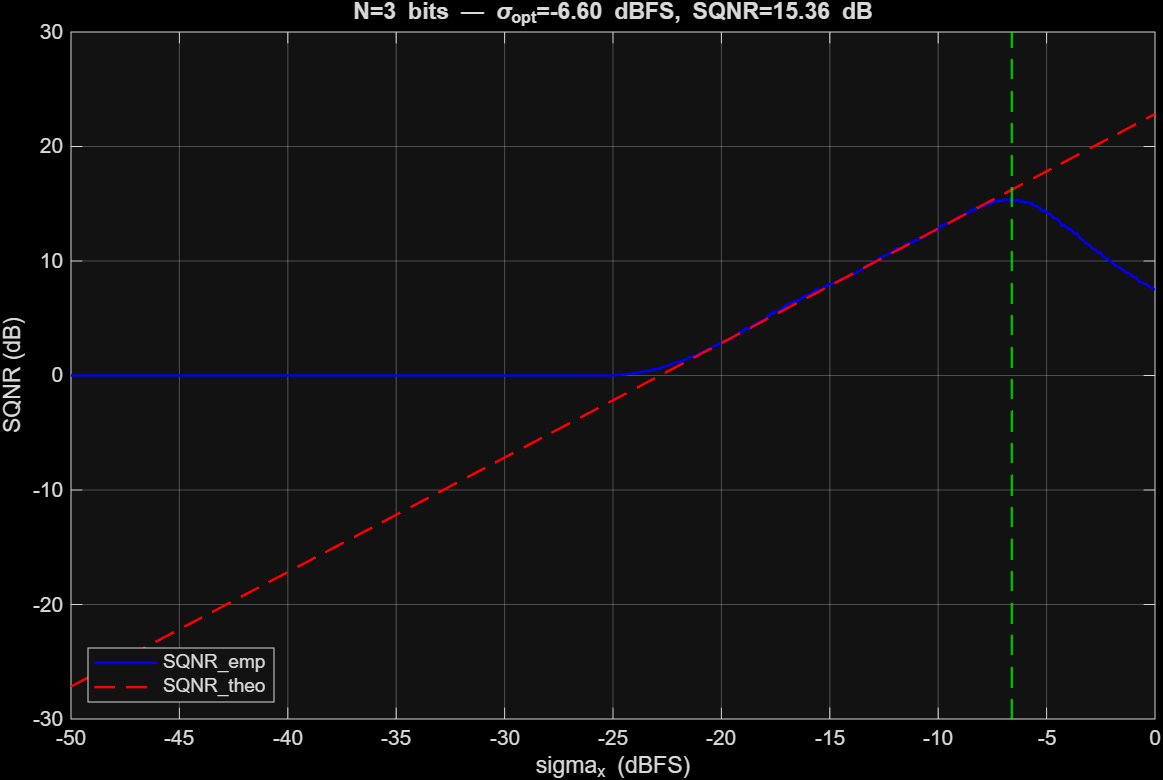
\includegraphics[width=\linewidth]{img/task3_tri_n3.png}
        \caption{N=3 bits - $\sigma_{opt}$=-6.60 dBFS, SQNR=15.36 dB}
    \end{subfigure}
    \hfill
    \begin{subfigure}[t]{.4\textwidth}
        \centering
        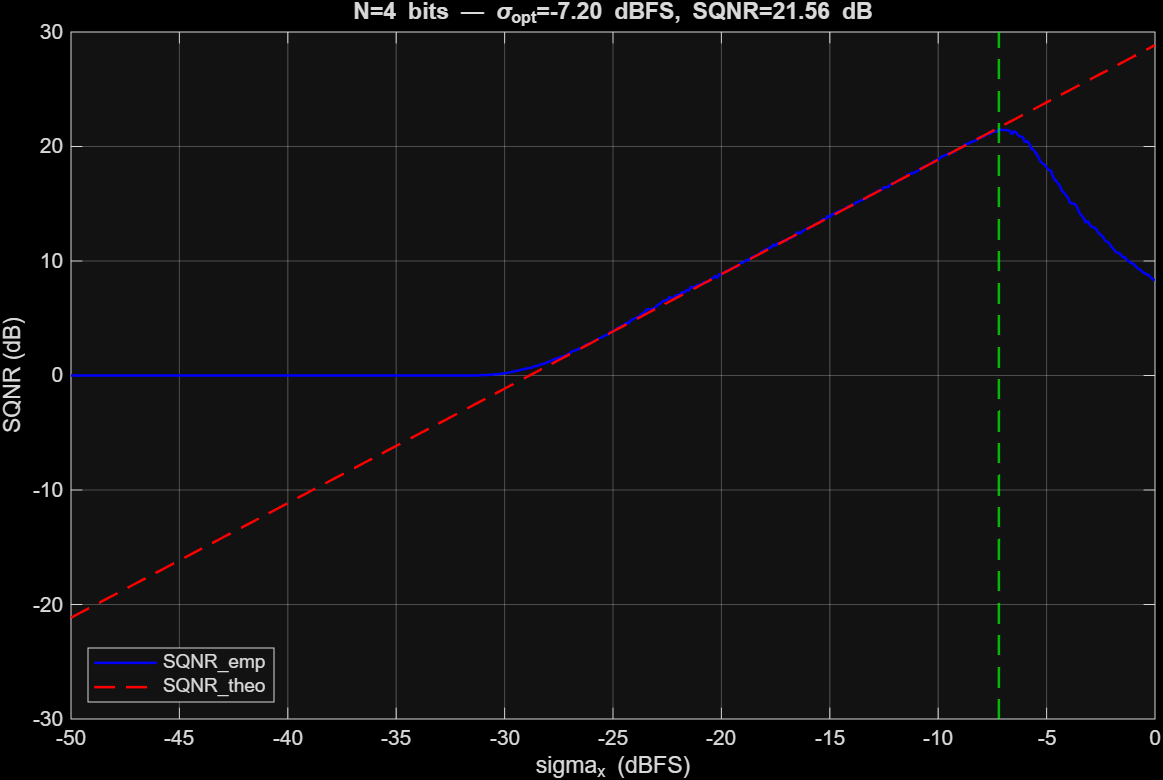
\includegraphics[width=\linewidth]{img/task3_tri_n4.png}
        \caption{N=4 bits - $\sigma_{opt}$=-7.20 dBFS, SQNR=21.56 dB}
    \end{subfigure}

    \medskip

    \begin{subfigure}[t]{.4\textwidth}
        \centering
        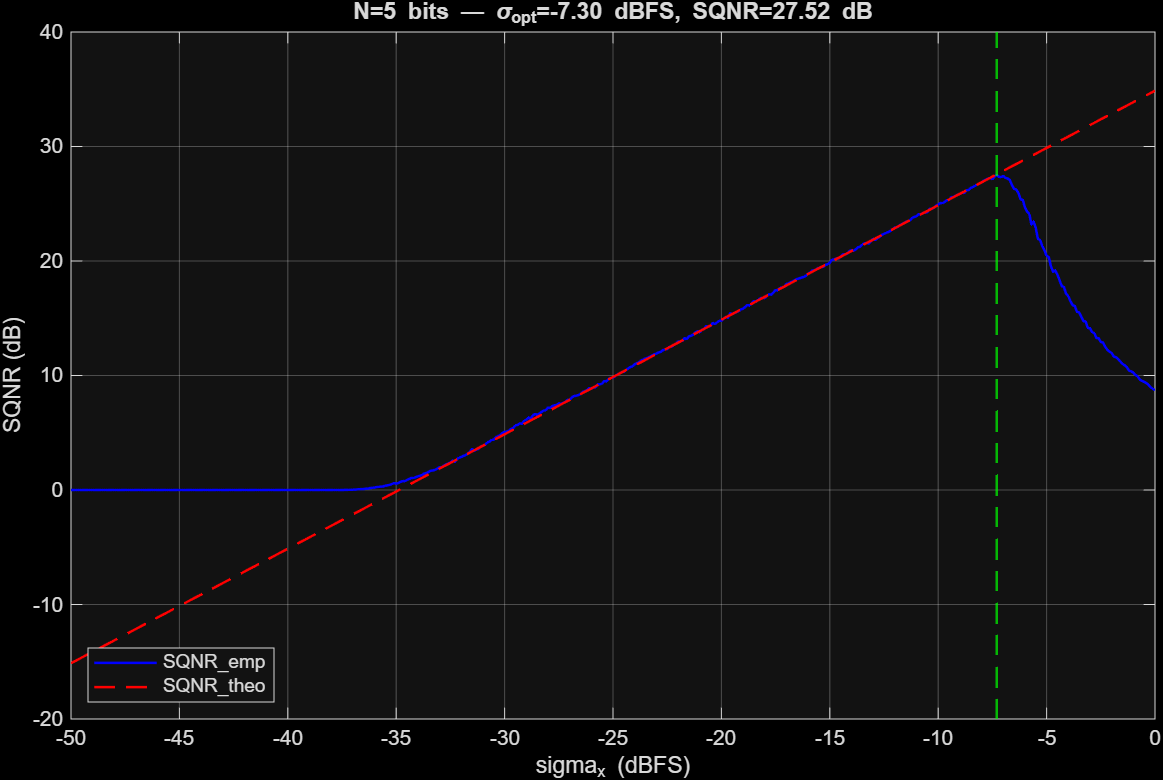
\includegraphics[width=\linewidth]{img/task3_tri_n5.png}
        \caption{N=5 bits - $\sigma_{opt}$=-7.30 dBFS, SQNR=27.52 dB}
    \end{subfigure}
    \hfill
    \begin{subfigure}[t]{.4\textwidth}
        \centering
        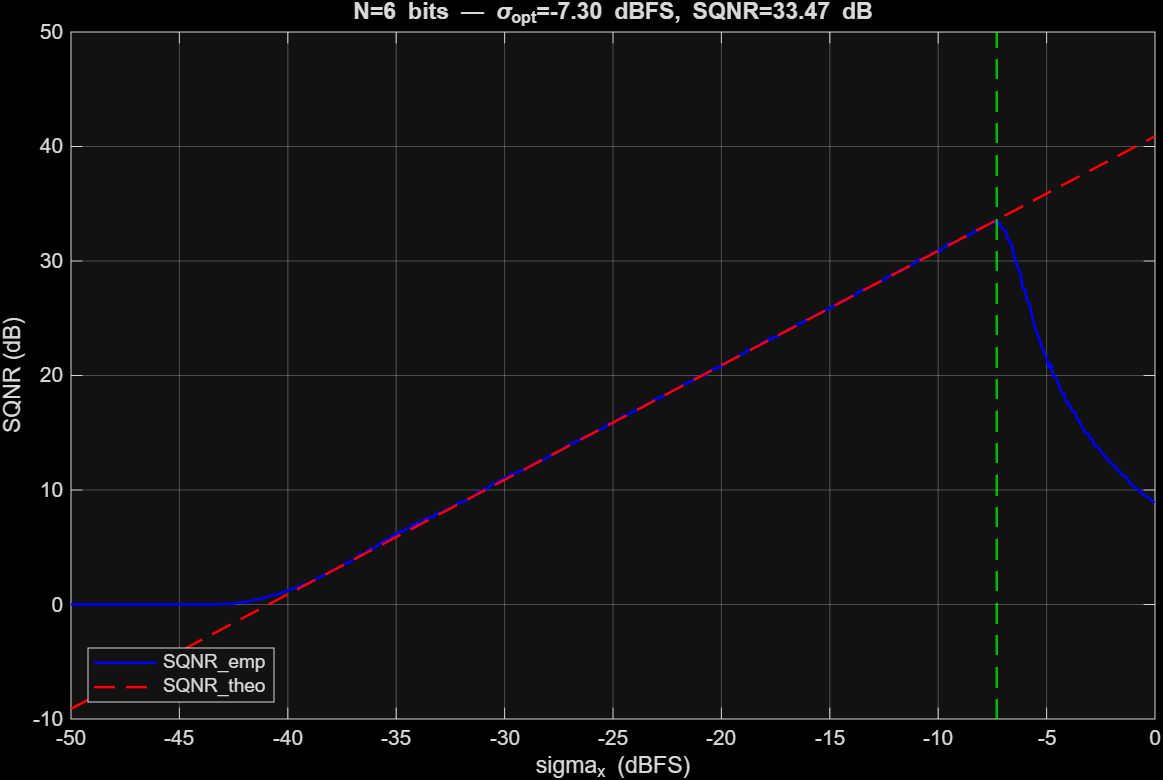
\includegraphics[width=\linewidth]{img/task3_tri_n6.png}
        \caption{N=6 bits - $\sigma_{opt}$=-7.30 dBFS, SQNR=33.47 dB}
    \end{subfigure}

    \caption{SQNR vs $\sigma_x$ (dBFS) for triangularly distributed input at different quantization resolutions.}
    \label{fig:task3_tri_sqnr_vs_sigma}
\end{figure}

The comparison between theoretical and empirical SQNR curves for triangularly distributed inputs is shown in Figure~\ref{fig:task3_tri_sqnr_vs_sigma}.
The red line represents the theoretical SQNR curve, while the blue line represents the empirical SQNR values obtained from quantizing the triangularly distributed samples.

Empirical curves deviate from the straight theoretical line for two practical reasons. At very small $\sigma_x$ values, quantization noise is no longer uniformly distributed and we have no enough bits for quantization.
At large $\sigma_x$ values, clipping occurs, distorting the signal and reducing SQNR below theoretical predictions.
Otherweise, in the mid-range of $\sigma_x$ values, empirical results closely follow theoretical expectations and reaches the maximum SQNR (marked in the description of each image).

When we increase the number of bits N, the curve starts to follow the theorical curve with smaller values of $\sigma_x$.
We reach a point where optimum $\sigma_x$ value (where SQNR is maximized) approaches the theoretical value of -7.78 dBFS calculated earlier.

\vspace{1cm}
\textbf{Question: In view of your results, what are the optimum values (regarding SQNR) of $\sigma_x$ (in dBFS), and for the different resolutions analyzed (3 to 6 bits)?
    Does this agree with your intuition (see first point above)?
}
\vspace{0.5cm}

ADD

\vspace{1cm}
\textbf{Question: Repeat the previous points, but now using normally distributed input samples with zero mean and standard deviation $\sigma_x$.
}
\vspace{0.5cm}

ADD

\vspace{0.5cm}
\section{Task 4}
\textbf{Assume a full-scale sinusoidal input with $f_0 = 37.1094 MHz$, and let the FFT size be M = 1024.
    Generate $15 \cdot M$ samples of $x(t)$ (at fs = 100 MHz) and quantize them to N = 12 bits. Break
    the vector xq of quantized samples into 15 size-M blocks using, e.g., the command reshape:}

\vspace{0.5cm}

\begin{lstlisting}[language=Matlab]
    xqblocks = reshape(xq, M, 15);
\end{lstlisting}

\textbf{so that each column of the $M \times 15$ matrix xqblocks will contain the corresponding block of size
    M . Now, since the fft command computes the FFT columnwise, in order to apply an M -point
    FFT to each block, we simply make
}
\begin{lstlisting}[language=Matlab]
    X = fft(xqblocks, M);
\end{lstlisting}

\textbf{Average the squared magnitude of the DFT coefficients over the 15 blocks and plot the results
    between 0 and fs/2, in dBFS.
    Observe the location and peak value of the principal frequency component, as well as the value
    of the noise floor. Do your observations agree (quantitatively) with what you would expect?
}

\vspace{0.5cm}
\section{Task 5}
\textbf{Question: Plot $g_\gamma(x)$ vs. $x$ in the range $x\in [-{\rm FS},{\rm FS}]$ for $\gamma = 0$, $1$ and $2$. For input signals whose values are always much smaller than $\rm FS$ (in absolute value), what will be the effect of the nonlinearity?
}
\vspace{0.5cm}

For inputs with amplitude much smaller than \(FS\), the nonlinearity \(g_{\gamma}(x)\) acts essentially as a constant gain: using $\lim_{\gamma \to 0} g_{\gamma}(x) = x$.
Thus, for \(|x|\ll FS\) the block only rescales the signal (no significant harmonic distortion) and the quantiser that follows sees an almost linearly amplified input. Significant compression and distortion appear only when \(|x|\) becomes a noticeable fraction of \(FS\).

\begin{figure}[H]
    \centering
    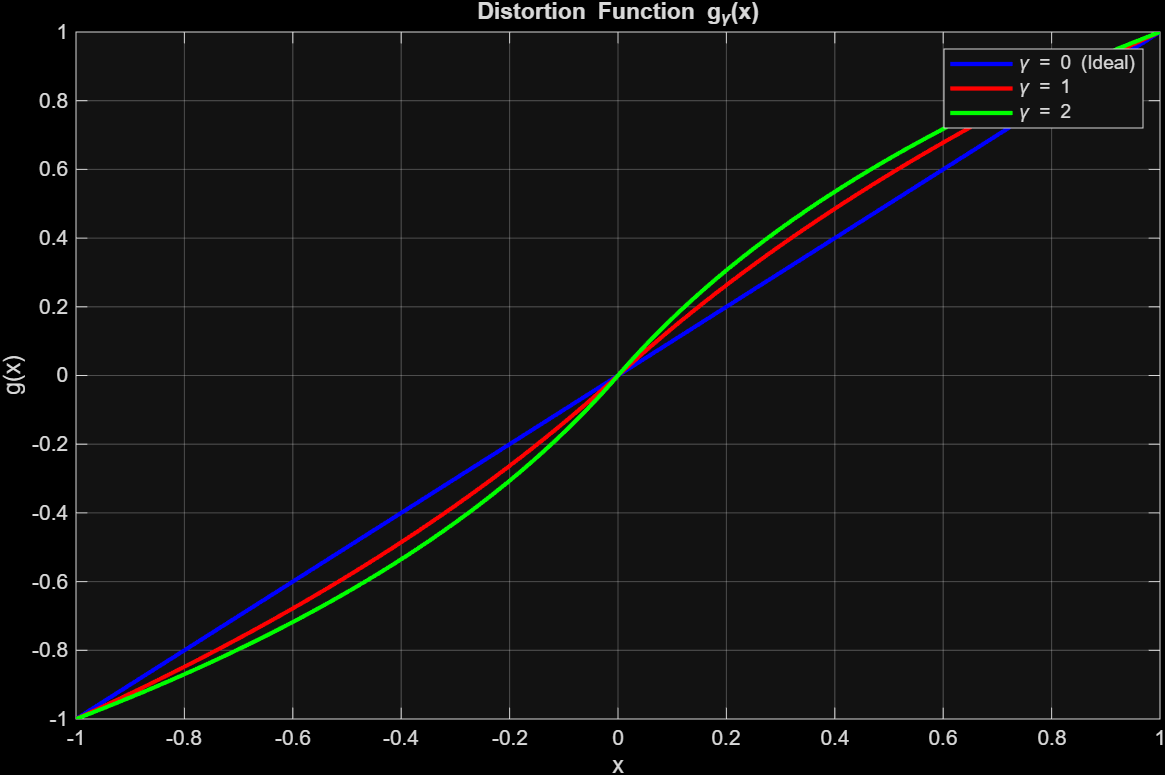
\includegraphics[width=1\textwidth]{img/task5_1.png}
    \label{fig:task5_1}
\end{figure}

\vspace{1cm}
\textbf{Question: Modify the code in {\tt quanti.m} and write a Matlab function {\tt dquanti.m} implementing this nonuniform quantizer. The format should be similar to that of {\tt quanti.m}, but including an additional input parameter {\tt gama}:}
\begin{center}
{\tt xq = dquanti( x, FS, Nbits, gama ); }
\end{center} 
\vspace{0.5cm}

We modified the function {\tt dquanti.m} as requested, if we receive \texttt{gama=0} the function behaves as a uniform quantizer, otherwise it applies the non-linear distortion before quantization.

The code is as follows:
\begin{lstlisting}[language=Matlab]
    function y = dquanti(x, FS, Nbits, gama)
    if gama == 0
        g_x = x; % Si gama=0, no hay distorsion (g(x) = x)
    else
        g_x = sign(x) .* (FS / log(1 + gama)) .* log(1 + gama .* abs(x) / FS);
        g_x(x == 0) = 0;
    end

    FS    = abs(FS);
    FSbin = 2^(Nbits-1);
    LSB   = FS/FSbin;  

        y = round(g_x/LSB); 
        y = min(y, FSbin-1); 
        y = max(y, -FSbin); 
        y = y * LSB;
\end{lstlisting}

\vspace{1cm}
\textbf{Question: Generate  samples (at 100 MHz) of a full-scale sinusoid with $f_0 = 6.8359$ MHz.
Quantize them to $N=11$ bits using $\gamma = 0.003$ in {\tt dquanti}. 
Determine the SFDR in dBFS using an FFT size $M=2048$, and then with $M=512$. 
Does the SFDR depend on the FFT size? Does the noise floor depend on the FFT size? How do you explain this?
}
\vspace{0.5cm}

We obtain the SFDR values from the FFT plots shown in Figures~\ref{fig:task5_2048} and~\ref{fig:task5_512}.
The SFDR values are:
\begin{itemize}
    \item For \(M=2048\): SFDR -71.3586 dBFS
    \item For \(M=512\): SFDR -71.2428 dBFS
\end{itemize}

For both $M=2048$ and $M=512$, the FFT of the quantized 11-bit sinusoid ($f_0=6.8359$\,MHz, $\gamma=0.003$) shows almost the same main harmonic and a largest spur.
Increasing the FFT size only reveals more detail in the lower part of the spectrum but does not change the SFDR value itself.

\begin{figure}[H]
    \centering
    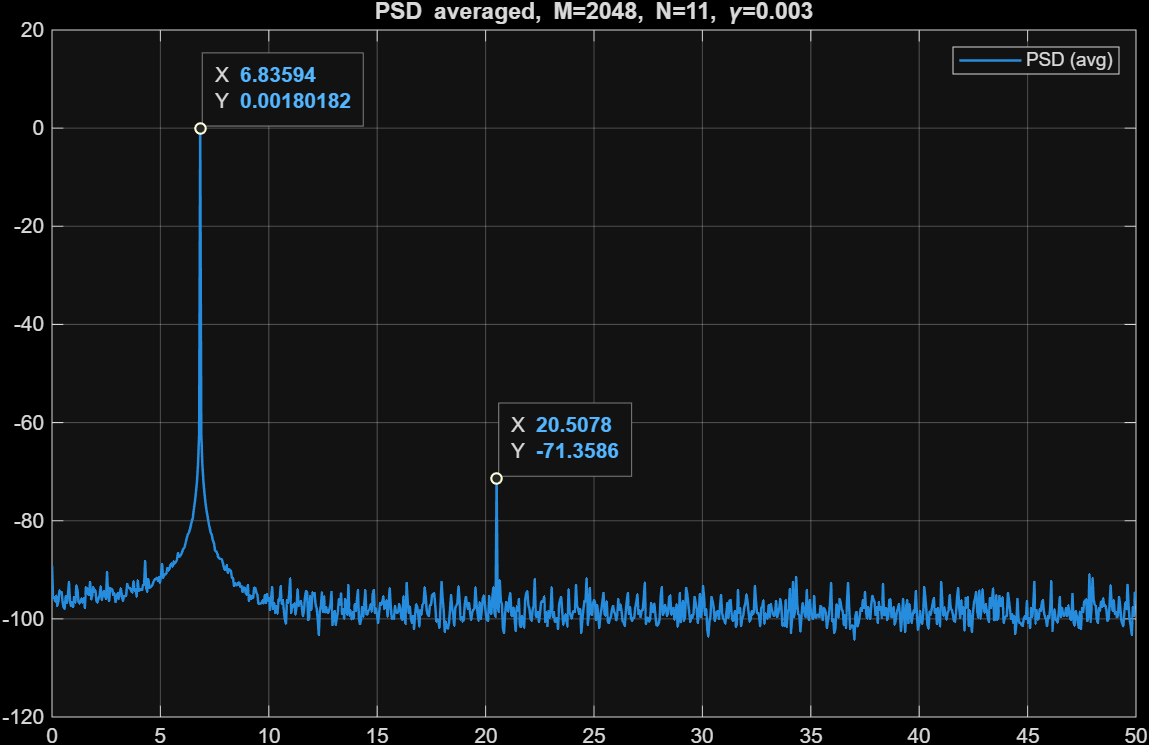
\includegraphics[width=1\textwidth]{img/task5_2048.png}
    \caption{FFT with $M=2048$, $N=11$, $\gamma=0.003$}
    \label{fig:task5_2048}
\end{figure}

\begin{figure}[H]
    \centering
    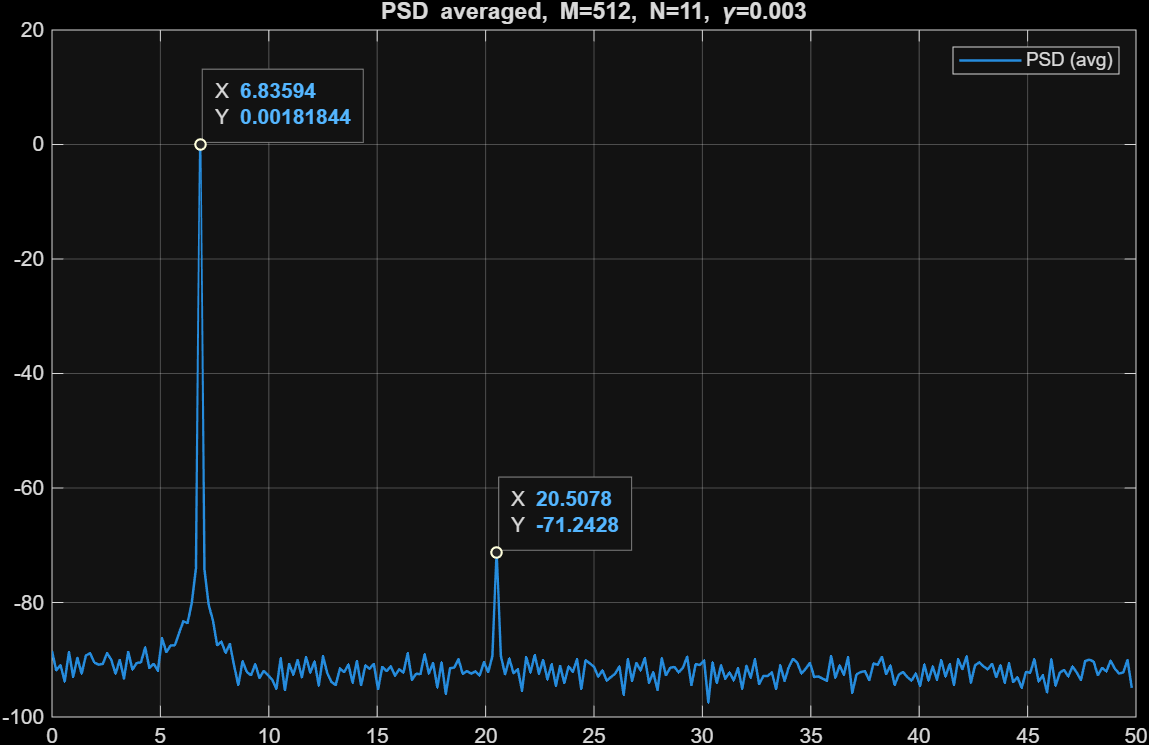
\includegraphics[width=1\textwidth]{img/task5_512.png}
    \caption{FFT with $M=512$, $N=11$, $\gamma=0.003$}
    \label{fig:task5_512}
\end{figure}

\vspace{1cm}
\textbf{Question: Using $M=2048$, repeat the previous step for $\gamma = 0.01$ and $0.1$. Are the spectral spurs located where you would expect?
}
\vspace{0.5cm}

From the FFT plots in Figures~\ref{fig:task5_y_0_01} and~\ref{fig:task5_y_0_1}, we can observe that as $\gamma$ increases, the amplitude of the distortion components (spurs) also increases.
For $\gamma = 0.01$, the spurs appear at the expected harmonic frequencies of the input tone, while for $\gamma = 0.1$ they become much more pronounced and clearly visible.

This confirms that the nonlinearity introduced by the companding function $g_\gamma(x)$ generates harmonic distortion.
The stronger the nonlinearity (larger $\gamma$), the greater the amplitude of these harmonics and the lower the SFDR.

\begin{figure}[H]
    \centering
    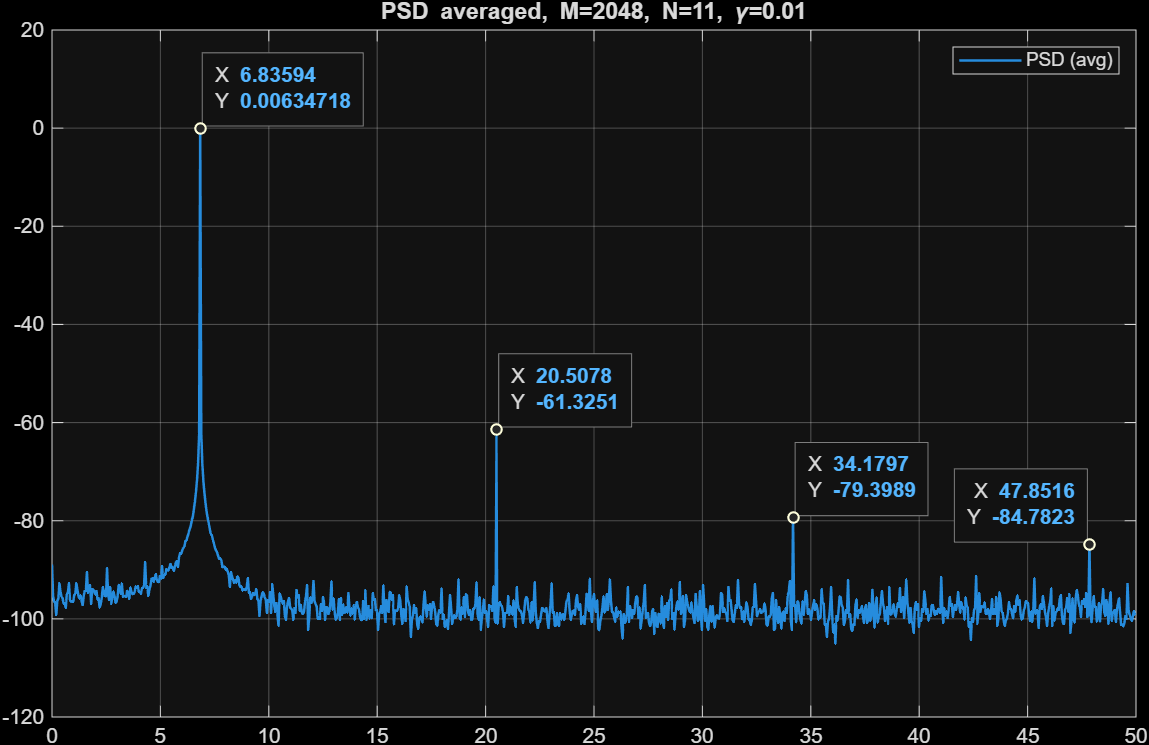
\includegraphics[width=1\textwidth]{img/task5_y_0_01.png}
    \caption{FFT with $M=2048$, $N=11$, $\gamma=0.01$}
    \label{fig:task5_y_0_01}
\end{figure}

\begin{figure}[H]
    \centering
    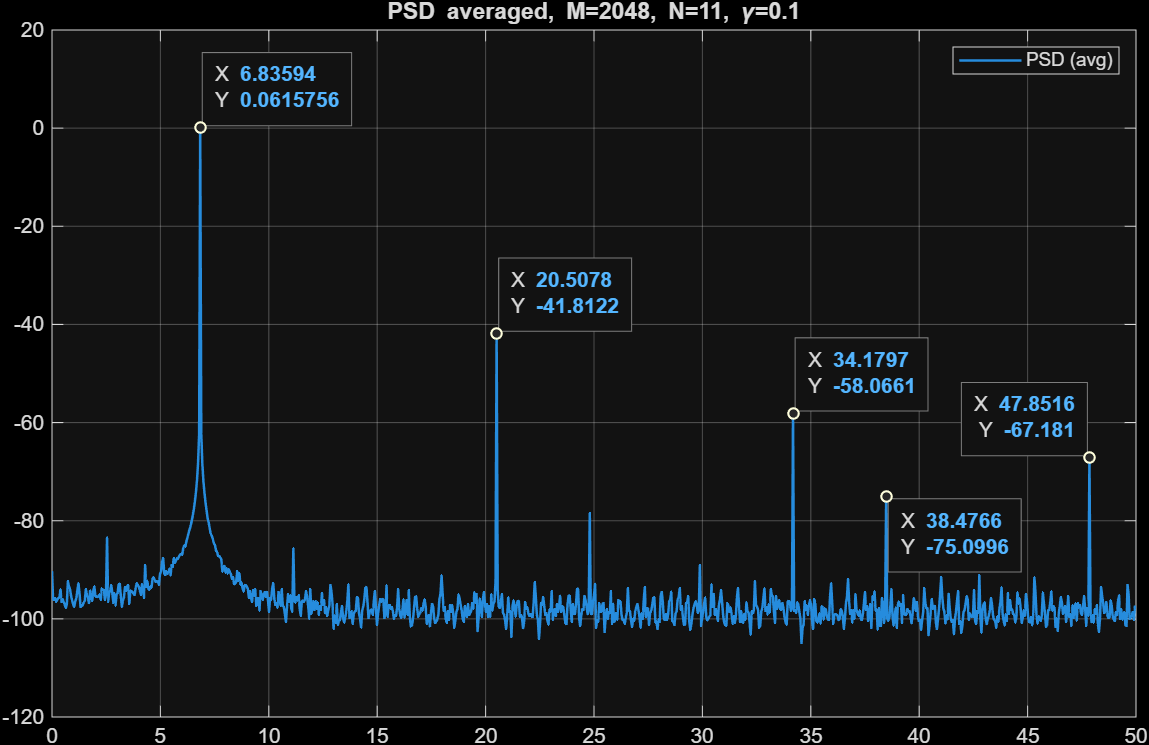
\includegraphics[width=1\textwidth]{img/task5_y_0_1.png}
    \caption{FFT with $M=2048$, $N=11$, $\gamma=0.1$}
    \label{fig:task5_y_0_1}
\end{figure}

\vspace{1cm}
\textbf{Question: Set now the amplitude to $\frac{\rm FS}{3}$. Using $M=2048$, measure the SFDR and express it in both dBFS and dBc for $\gamma=0.005$, $0.05$ and $0.1$. Will these values change if you repeat the analysis with $M=512$?
}
\vspace{0.5cm}

From Figure~\ref{fig:task5_5}, we can see that when the input amplitude is reduced to $\frac{\mathrm{FS}}{3}$, the fundamental tone decreases while the relative amplitude of the spurious components (spurs) remains almost unchanged.
This causes the SFDR values, both in dBFS and dBc, to be slightly worse than in the full-scale case.

As $\gamma$ increases, the nonlinearity becomes stronger and the harmonic distortion more evident, especially for $\gamma = 0.1$.
The comparison between $M = 2048$ and $M = 512$ shows that the FFT size does not significantly change the SFDR value; it only affects the frequency resolution, making the spectrum appear smoother and more detailed for higher $M$.

\begin{figure}[H]
  \centering
  % fila 1 (3 imágenes)
  \begin{subfigure}[t]{0.45\textwidth}
    \centering
    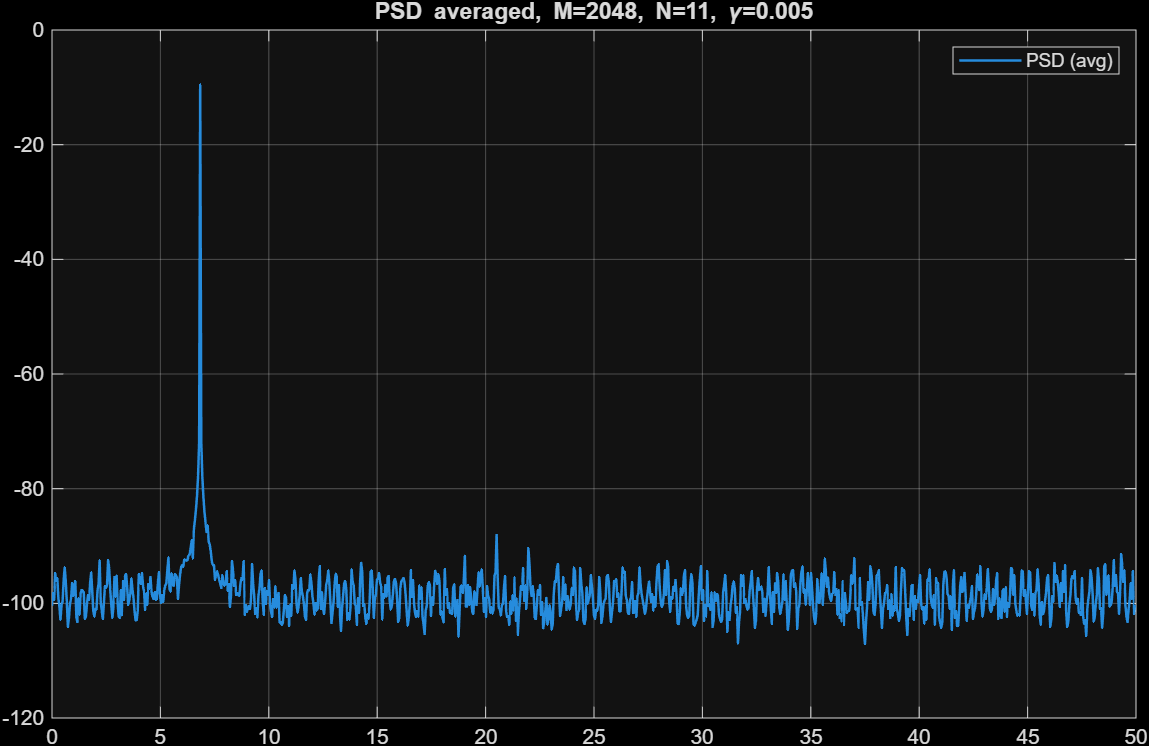
\includegraphics[width=\linewidth,height=0.28\textheight,keepaspectratio]{img/task5_5_1.png}
    \caption{FFT with $M=2048$, $N=11$, $\gamma=0.005$}
  \end{subfigure}\hfill
  \begin{subfigure}[t]{0.45\textwidth}
    \centering
    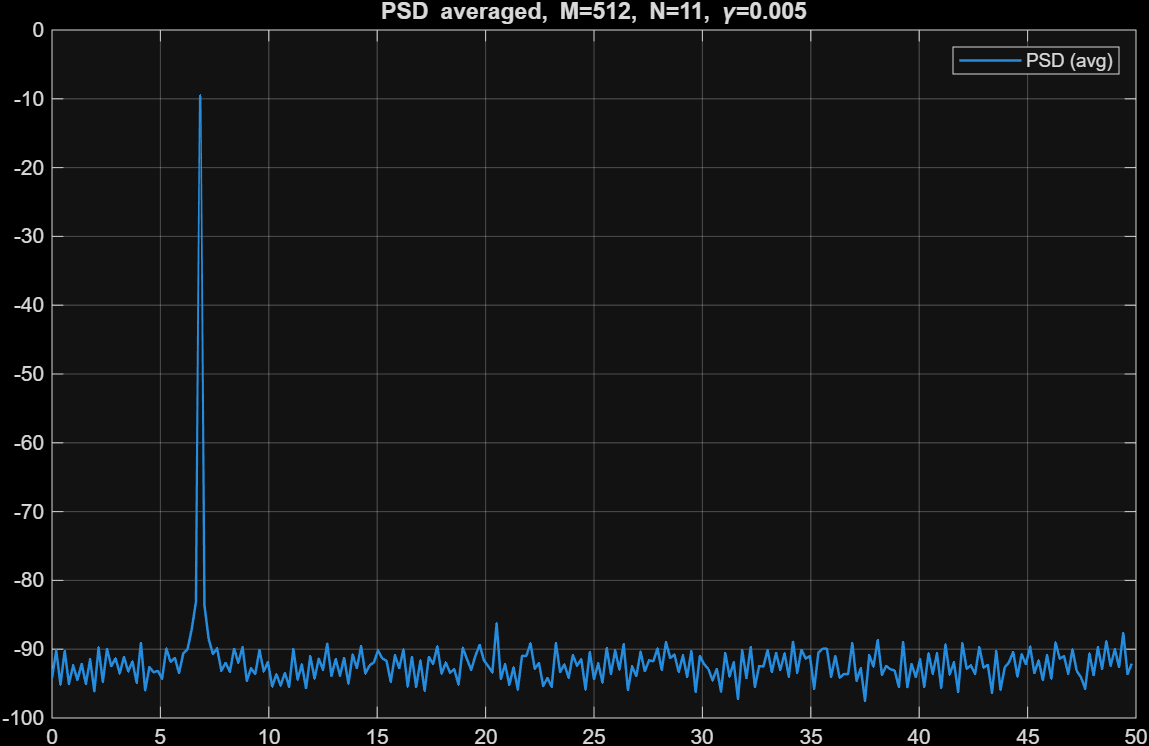
\includegraphics[width=\linewidth,height=0.28\textheight,keepaspectratio]{img/task5_5_4.png}
    \caption{FFT with $M=512$, $N=11$, $\gamma=0.005$}
  \end{subfigure}

  \vspace{1ex}

  \begin{subfigure}[t]{0.45\textwidth}
    \centering
    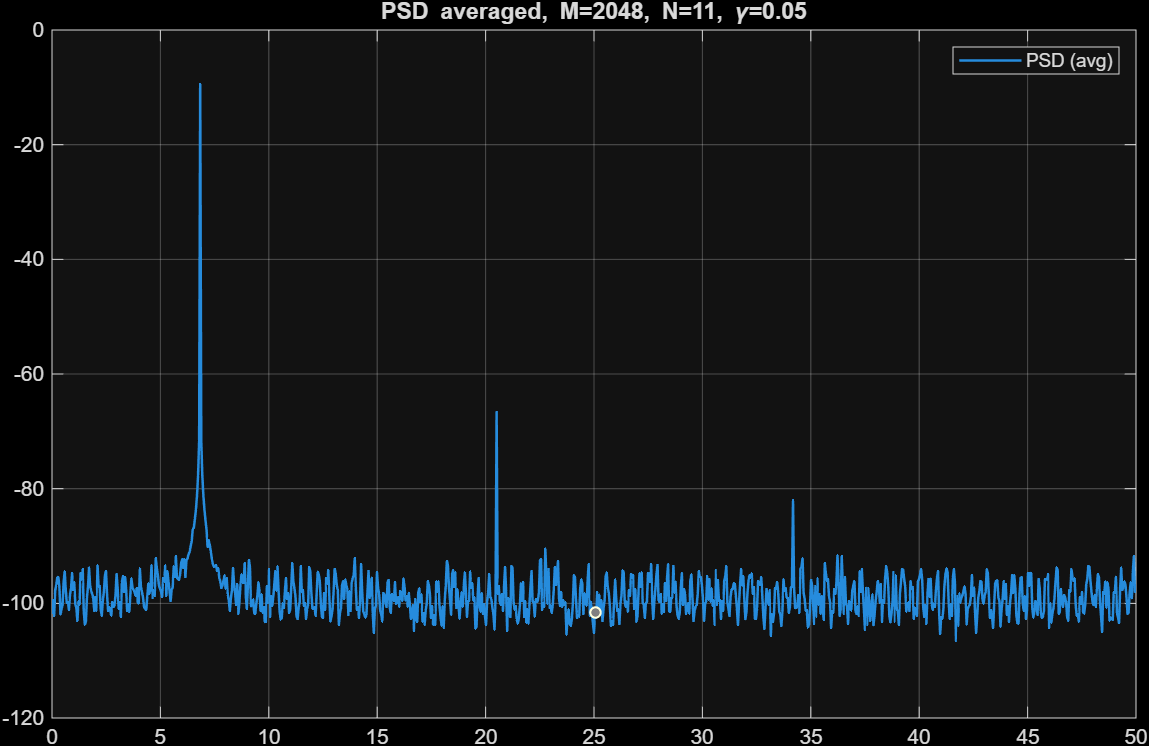
\includegraphics[width=\linewidth,height=0.28\textheight,keepaspectratio]{img/task5_5_2.png}
    \caption{FFT with $M=2048$, $N=11$, $\gamma=0.05$}
  \end{subfigure}\hfill
  \begin{subfigure}[t]{0.45\textwidth}
    \centering
    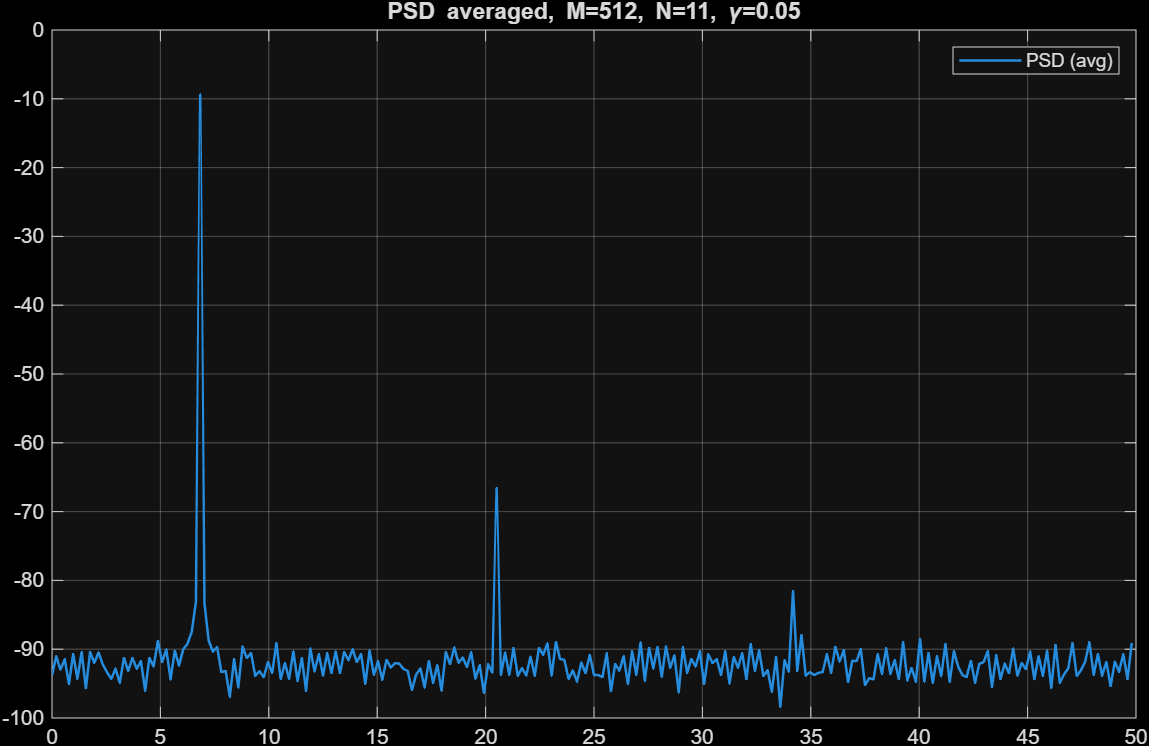
\includegraphics[width=\linewidth,height=0.28\textheight,keepaspectratio]{img/task5_5_5.png}
    \caption{FFT with $M=512$, $N=11$, $\gamma=0.05$}
  \end{subfigure}

  \vspace{1ex}

  \begin{subfigure}[t]{0.45\textwidth}
    \centering
    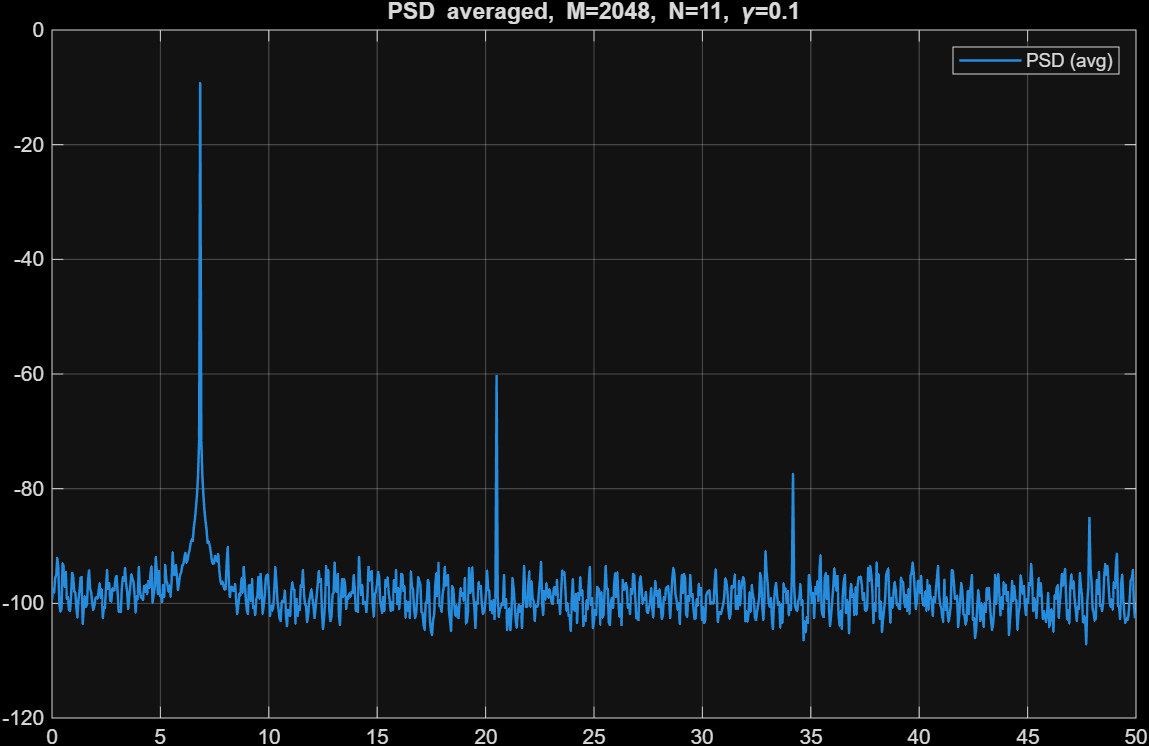
\includegraphics[width=\linewidth,height=0.28\textheight,keepaspectratio]{img/task5_5_3.png}
    \caption{FFT with $M=2048$, $N=11$, $\gamma=0.1$}
  \end{subfigure}\hfill
  \begin{subfigure}[t]{0.45\textwidth}
    \centering
    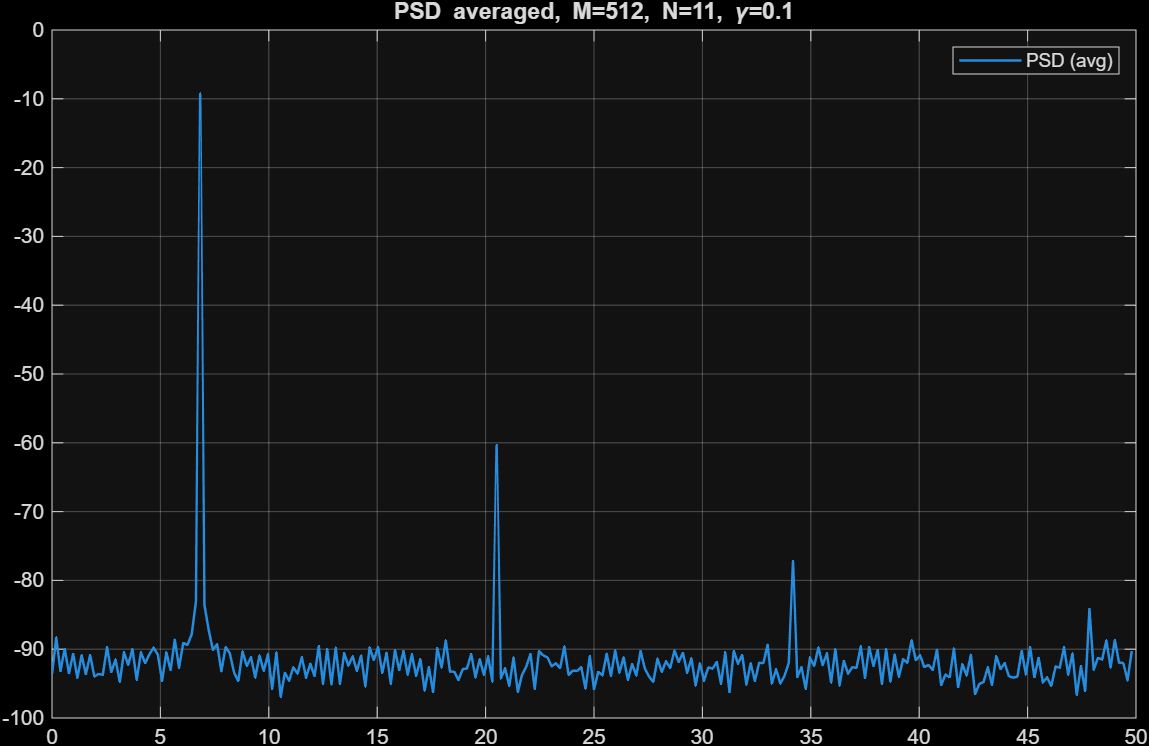
\includegraphics[width=\linewidth,height=0.28\textheight,keepaspectratio]{img/task5_5_6.png}
    \caption{FFT with $M=512$, $N=11$, $\gamma=0.1$}
  \end{subfigure}

  \caption{FFTs with different $M$ values, $N=11$, and varying $\gamma$.}
  \label{fig:task5_5}
\end{figure}

\vspace{1cm}
\textbf{Question: Consider now samples (at 100 MHz and with 11-bit resolution) of a sinusoid with frequency $3.3202$ MHz and amplitude $\frac{\rm FS}{2}$. Obtain the THD for this nonuniform ADC with $\gamma = 0.3$ under the IEEE 1241-2000 specification, expressed in both dB and percentage.
}
\vspace{0.5cm}

We only got 7 armonics above the noise floor in the FFT plot shown in Figure~\ref{fig:task5_thd}, so we calculated the THD using these harmonics.
The other armonics appear past the 50 MHz marked.

\begin{figure}[H]
    \centering
    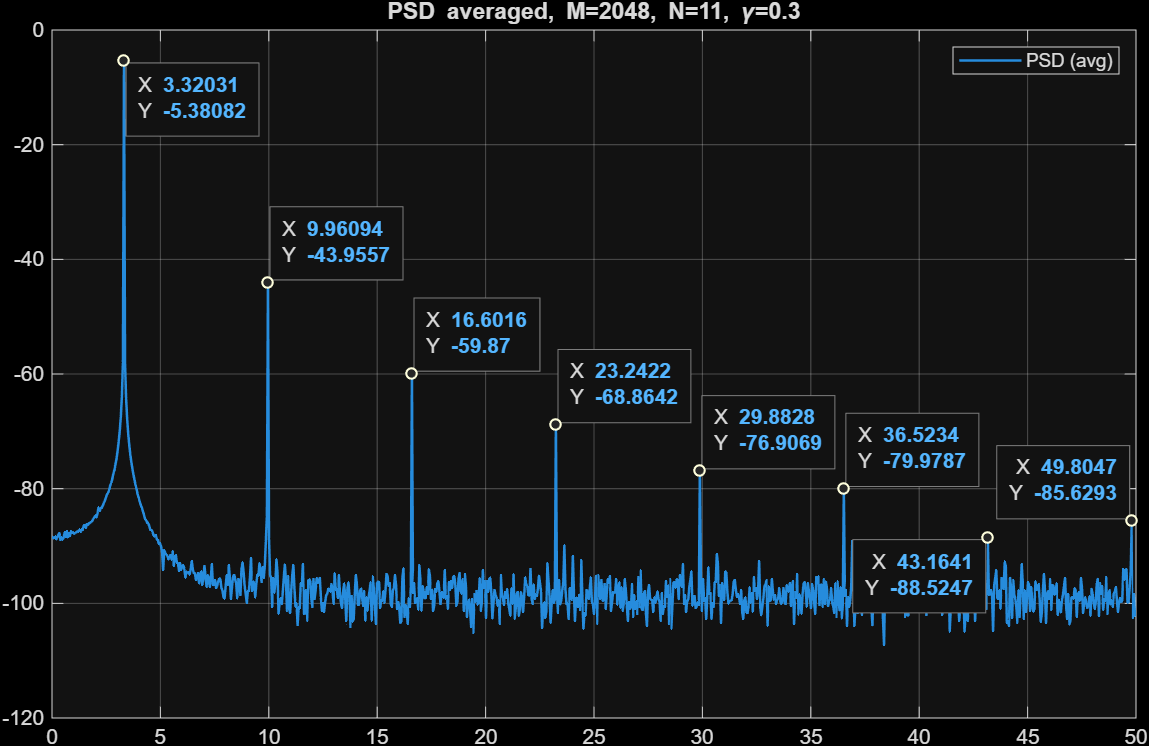
\includegraphics[width=1\textwidth]{img/task5_thd.png}
    \caption{FFT with $M=2048$, $N=11$, $\gamma=0.3$}
    \label{fig:task5_thd}
\end{figure}

The Total Harmonic Distortion (THD) according to the IEEE 1241-2000 specification is defined as:

\[
\mathrm{THD} = 10 \log_{10}
\left(
    \frac{A_2^2 + A_3^2 + \cdots + A_{10}^2}{A_1^2}
\right) \, \mathrm{[dB]}
\]

where \(A_1\) is the amplitude of the fundamental component, and \(A_2, A_3, \ldots, A_{10}\) are the amplitudes of the first nine harmonics.

From the measured spectrum, the obtained value is:

\[
\mathrm{THD} = 2,44~\mathrm{dB}
\]


\vspace{0.5cm}
\section{Task 6}
\textbf{Question: If the rms value of the aperture jitter is 20 ps, and the input signal is a full-scale sinusoid with frequency $f_c$,
    for which values of $f_c$ will the aperture error power dominate the quantization noise power?
}
\vspace{0.5cm}

$SQNR = 20 * log_{10}(1 / (2*\pi*fc*\sigma))$

$fc = 1 / ( 10^(SQNR / 20) * 2*\pi*\sigma $

$fc$ should be greater than $1 / ( 10^(SQNR / 20) * 2*\pi*\sigma $

\vspace{1cm}
\textbf{Question: If the rms value of the aperture jitter is 20 ps, and the input signal is a 3-MHz sinusoid, for which values of the amplitude
    (in dBFS) will the aperture error power dominate the quantization noise power?
}
\vspace{0.5cm}

$\sigma_{q}^{2}=\frac{\Delta^{2}}{12}$.

$\Delta=\frac{2\cdot FS}{2^{N}}$

$\sigma_{q}^{2} = \frac{1}{12} \left( \frac{2 \cdot FS}{2^N} \right)^2 = \frac{FS^2}{3 \cdot (2^N)^2}$

$\sigma_e^2 > \sigma_q^2$

$A_{dBFS} > 66.71 - 6.02 \cdot N$


\vspace{1cm}
\textbf{Question: Simulate the effect of aperture jitter on a full-scale sinusoid with frequency $40.03905$ MHz.
    Consider two cases: $\sigma_\tau = 10$ ps and $\sigma_\tau=0.1$ ps respectively.
    Perform a 1024-FFT analysis of your data and check whether the perceived noise floor is at the expected level.
}
\vspace{0.5cm}

For $\sigma_\tau = 10ps$, the noise floor is-79.1 DBFS, and for  $\sigma_\tau = 0,1ps$ is -101 DBFS

\begin{figure}[H]
    \begin{subfigure}[t]{.5\textwidth}
        \centering
        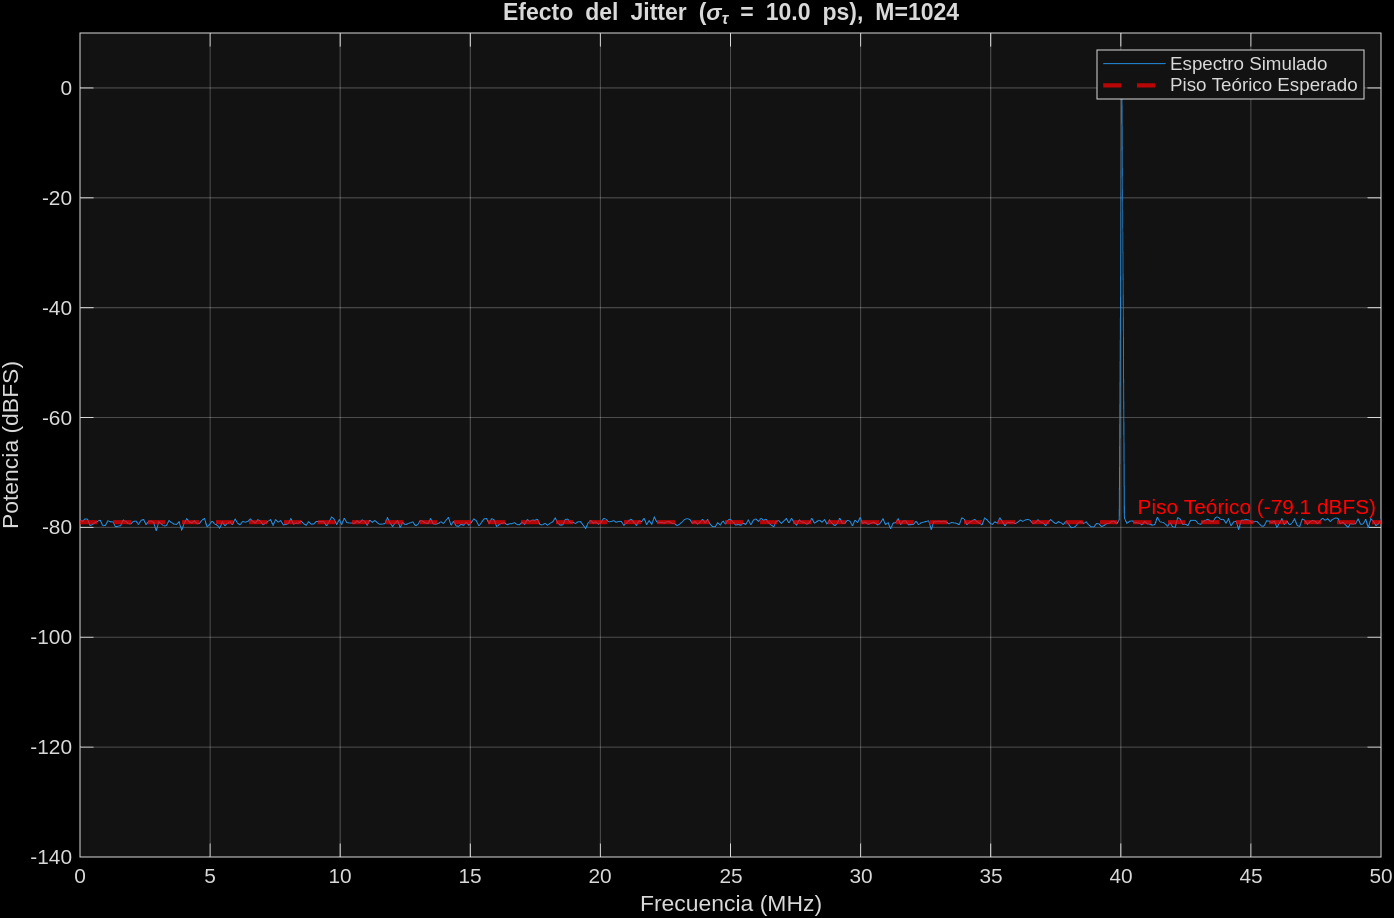
\includegraphics[width=\linewidth]{img/task6_3_10ps.png}
        \caption{$\sigma_\tau = 10ps$}
    \end{subfigure}
    \begin{subfigure}[t]{.5\textwidth}
        \centering
        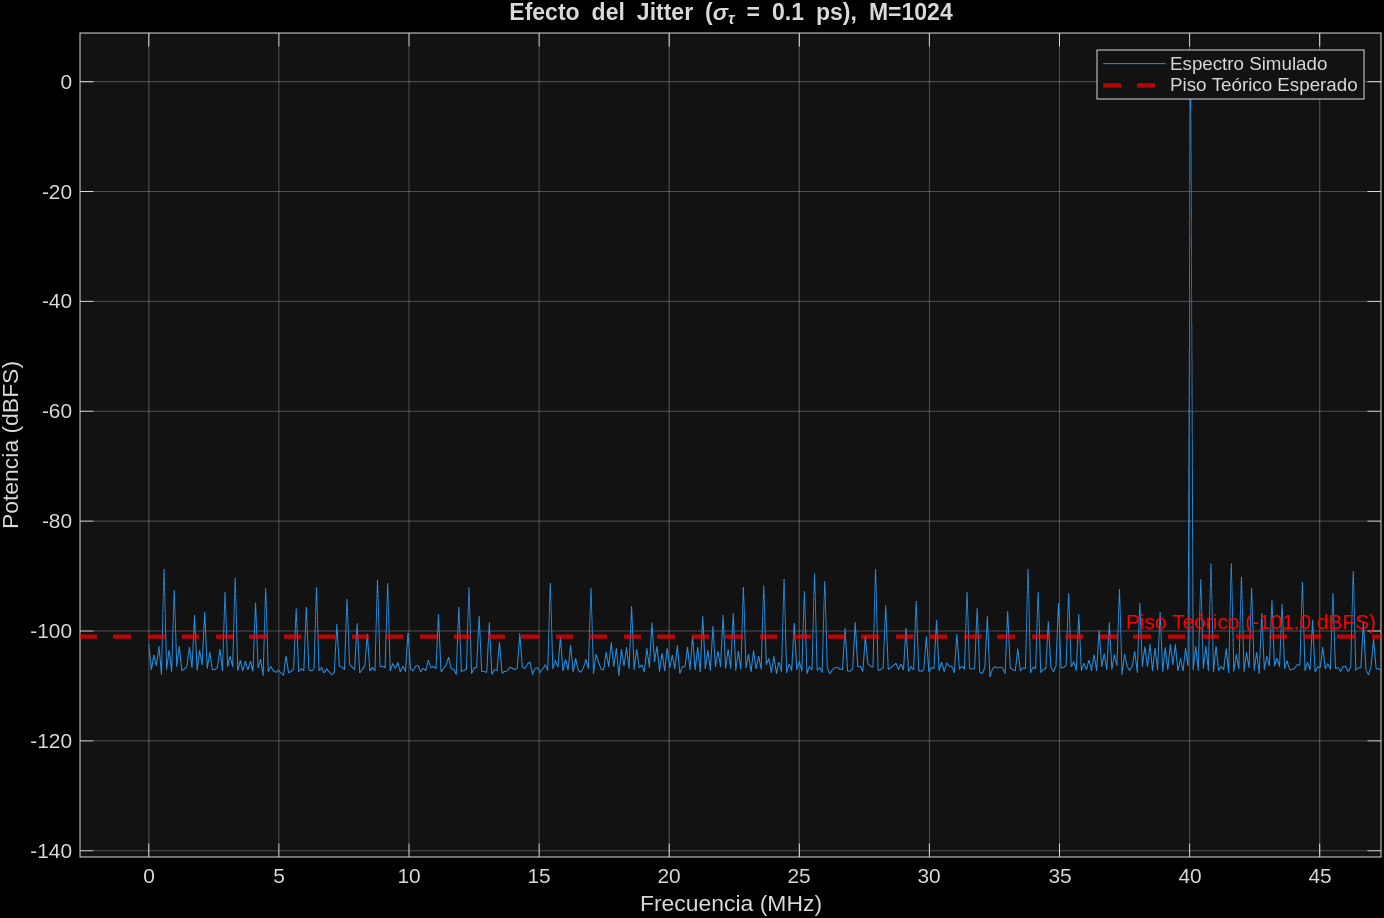
\includegraphics[width=\linewidth]{img/task6_3_01ps.png}
        \caption{$\sigma_\tau = 0,1ps$}
    \end{subfigure}

\end{figure}

\vspace{1cm}
\textbf{Question: Neglecting other possible sources of distortion, the total SNR is given by the ratio of the signal
    power to the sum of the powers of the noises due to jitter and quantization. Plot the theoretical total SNR (in dB) vs.
    input frequency over the range 0.1--100 MHz, assuming a full-scale sinusoid and for $\sigma_\tau \in \{10,20,40\}$ ps,
    $N\in \{10, 14\}$ bits (so that you should have six graphs in a single plot, whose x-axis should be in log scale).
    Comment on your results.
}
\vspace{0.5cm}

xd



\end{document}